\documentclass[8pt,aspectratio=1610]{beamer}
\usepackage[utf8]{inputenc}
\usepackage{booktabs}
\usepackage{array}
\usepackage{graphicx}
\usepackage{xcolor}
\usepackage{tikz}
\usetikzlibrary{positioning,arrows.meta,decorations.pathreplacing,calc,shadows}

% TikZ styles for neural networks
\tikzset{
    neuron/.style={circle, draw, minimum size=1cm, inner sep=0pt, fill=white, drop shadow},
    input neuron/.style={neuron, fill=inputcolor!30, draw=inputcolor!70},
    hidden neuron/.style={neuron, fill=hiddencolor!30, draw=hiddencolor!70},
    output neuron/.style={neuron, fill=outputcolor!30, draw=outputcolor!70},
    bias neuron/.style={neuron, fill=biascolor!30, draw=biascolor!70},
    small neuron/.style={neuron, minimum size=0.7cm},
    large neuron/.style={neuron, minimum size=1.3cm},
    weight/.style={->, thick},
    layer label/.style={font=\small\bfseries},
    connection/.style={->, thick, black!60},
    strong connection/.style={->, very thick, black!80},
    weak connection/.style={->, thin, black!40},
    activation/.style={rounded corners, draw, fill=yellow!20, minimum width=2cm, minimum height=0.8cm},
    function box/.style={rectangle, draw, fill=blue!10, minimum width=1.5cm, minimum height=0.6cm},
    computation/.style={rectangle, draw, fill=green!10, minimum width=1.2cm, minimum height=0.8cm},
    flow arrow/.style={->, very thick, blue!70},
    error arrow/.style={->, very thick, red!70},
    gradient arrow/.style={->, thick, orange!70, dashed}
}
\usepackage{pgfplots}
\pgfplotsset{compat=1.18}
\usepackage{amsmath}
\usepackage{amssymb}
\usepackage{amsfonts}
\usepackage{algorithm}
\usepackage{algorithmic}

\usetheme{metropolis}
\usecolortheme{wolverine}
\metroset{progressbar=frametitle,block=fill}
\setbeamertemplate{navigation symbols}{}

% Define custom colors complementing the Wolverine theme
\definecolor{maizelight}{RGB}{255, 203, 5}      % Light maize for examples
\definecolor{maizedark}{RGB}{255, 167, 0}       % Darker maize for emphasis
\definecolor{bluelight}{RGB}{0, 39, 76}         % Deep blue for blocks
\definecolor{tealaccent}{RGB}{0, 128, 128}      % Teal for variety
\definecolor{orangeaccent}{RGB}{255, 138, 51}   % Orange complement

% Neural network visualization colors
\definecolor{inputcolor}{RGB}{244, 67, 54}      % Red for input layer
\definecolor{hiddencolor}{RGB}{33, 150, 243}    % Blue for hidden layers
\definecolor{outputcolor}{RGB}{76, 175, 80}     % Green for output layer
\definecolor{biascolor}{RGB}{255, 193, 7}       % Amber for bias

% Customize block colors
\setbeamercolor{block title}{bg=bluelight,fg=white}
\setbeamercolor{block body}{bg=bluelight!10,fg=black}

% Example blocks in complementary maize
\setbeamercolor{block title example}{bg=maizelight,fg=black}
\setbeamercolor{block body example}{bg=maizelight!15,fg=black}

% Alert blocks in orange accent
\setbeamercolor{block title alerted}{bg=orangeaccent,fg=white}
\setbeamercolor{block body alerted}{bg=orangeaccent!15,fg=black}

% Create custom colored blocks for variety
\newenvironment<>{techblock}[1]{%
  \setbeamercolor{block title}{bg=tealaccent,fg=white}%
  \setbeamercolor{block body}{bg=tealaccent!10,fg=black}%
  \begin{block}#2{#1}}{\end{block}}

\newenvironment<>{tipblock}[1]{%
  \setbeamercolor{block title}{bg=maizedark,fg=black}%
  \setbeamercolor{block body}{bg=maizedark!15,fg=black}%
  \begin{block}#2{#1}}{\end{block}}

\title{Artificial Neural Networks}
\subtitle{CMSC 173 - Machine Learning}
\author{Course Lecture}
\date{}

\begin{document}

\begin{frame}
\titlepage
\end{frame}

\begin{frame}{Outline}
\tableofcontents
\end{frame}

% ========================================
% Section: Introduction
% ========================================

\section{Introduction \& Motivation}

\begin{frame}{What Are Neural Networks?}
\centering
\textbf{Artificial Neural Networks: Computing systems inspired by biological neural networks}

\vspace{0.3cm}

\begin{columns}[t]
\begin{column}{0.48\textwidth}
\begin{block}{Biological Inspiration}
\begin{itemize}
\setlength{\itemsep}{3pt}
\item \textbf{Neurons}: Basic processing units
\item \textbf{Synapses}: Weighted connections
\item \textbf{Learning}: Adapting connection strengths
\item \textbf{Parallel processing}: Massive connectivity
\end{itemize}
\end{block}
\end{column}

\begin{column}{0.48\textwidth}
\begin{block}{Artificial Counterpart}
\begin{itemize}
\setlength{\itemsep}{3pt}
\item \textbf{Perceptrons}: Mathematical neurons
\item \textbf{Weights}: Learnable parameters
\item \textbf{Training}: Gradient-based optimization
\item \textbf{Layers}: Organized processing units
\end{itemize}
\end{block}
\end{column}
\end{columns}

\vspace{0.2cm}

\begin{alertblock}{Key Insight}
Neural networks can \textbf{learn complex non-linear mappings} from data by adjusting weights through training.
\end{alertblock}
\end{frame}

\begin{frame}{Why Neural Networks?}
\textbf{Motivation: Limitations of Linear Models}

\vspace{0.2cm}

\begin{columns}[t]
\begin{column}{0.48\textwidth}
\begin{block}{Linear Models}
\begin{itemize}
\setlength{\itemsep}{3pt}
\item Limited to linear decision boundaries
\item Cannot solve XOR problem
\item Restricted representational power
\item Simple but insufficient for complex data
\end{itemize}
\end{block}

\textbf{Example: XOR Problem}
\begin{center}
\begin{tabular}{cc|c}
$x_1$ & $x_2$ & XOR \\
\hline
0 & 0 & 0 \\
0 & 1 & 1 \\
1 & 0 & 1 \\
1 & 1 & 0 \\
\end{tabular}
\end{center}
\textcolor{red}{No linear classifier can solve this!}
\end{column}

\begin{column}{0.48\textwidth}
\begin{block}{Neural Networks}
\begin{itemize}
\setlength{\itemsep}{3pt}
\item Non-linear decision boundaries
\item Universal approximation capability
\item Hierarchical feature learning
\item Scalable to complex problems
\end{itemize}
\end{block}

\textbf{Universal Approximation Theorem:}
A neural network with a single hidden layer can approximate any continuous function to arbitrary accuracy (given sufficient neurons).

\vspace{0.2cm}

\textbf{Key Advantages:}
\begin{itemize}
\item Automatic feature extraction
\item End-to-end learning
\item Flexible architectures
\end{itemize}
\end{column}
\end{columns}
\end{frame}

% ========================================
% Section: The Perceptron
% ========================================

\section{The Perceptron}

\begin{frame}{The Perceptron: Building Block of Neural Networks}
\centering

\begin{tikzpicture}[scale=1.0, every node/.style={scale=1.0}]
    % Input nodes - better vertical spacing and centered
    \node[input neuron] (x1) at (0,2.5) {$x_1$};
    \node[input neuron] (x2) at (0,1.5) {$x_2$};
    \node[input neuron] (x3) at (0,0.5) {$x_3$};
    \node[bias neuron] (x0) at (0,-0.5) {$x_0$};
    % \node[above=0.05cm of x0, font=\tiny] {bias};

    % Intermediate processing nodes - better horizontal alignment
    \node[computation] (sum) at (3.5,1) {$\sum$};
    \node[activation] (sigma) at (5.5,1) {$\sigma$};

    % Output neuron - centered vertically with processing nodes
    \node[output neuron, large neuron] (y) at (7.5,1) {$y$};

    % Connections from inputs to summation with better routing
    \coordinate (sumIn) at (2.8,1);
    \draw[strong connection] (x1) -- (sumIn);
    \draw[strong connection] (x2) -- (sumIn);
    \draw[strong connection] (x3) -- (sumIn);
    \draw[strong connection] (x0) -- (sumIn);

    % Weight labels positioned clearly above connections
    \node at (1.4, 2.2) [font=\small] {$w_1$};
    \node at (1.4, 1.5) [font=\small] {$w_2$};
    \node at (1.4, 0.8) [font=\small] {$w_3$};
    \node at (1.4, 0.1) [font=\small] {$b$};

    % Flow arrows between processing stages
    \draw[flow arrow] (sum) -- (sigma);
    \draw[flow arrow] (sigma) -- (y);

    % Mathematical formulation - positioned below with consistent spacing
    \node[below=0.8cm of sum, font=\small] {$z = \sum_{i=1}^{n} w_i x_i + b$};
    \node[below=0.8cm of sigma, font=\small] {$y = \sigma(z)$};

    % Input and Output labels - better positioning
    \node[left=0.2cm of x1, font=\bfseries\small] {Inputs};
    \node[right=0.2cm of y, font=\bfseries\small] {Output};
\end{tikzpicture}

\vspace{0.2cm}

\begin{alertblock}{Mathematical Model}
\textbf{Linear Combination:} $z = \sum_{i=1}^{n} w_i x_i + b = \mathbf{w}^T\mathbf{x} + b$

\textbf{Activation:} $y = \sigma(z)$ where $\sigma$ is an activation function
\end{alertblock}
\end{frame}

\begin{frame}{Neural Network Components and Architecture}
\begin{columns}[t]
\begin{column}{0.48\textwidth}
\centering
\textbf{Single Processing Unit}

\vspace{0.3cm}

\begin{tikzpicture}[scale=0.8, every node/.style={scale=0.8}]
    % Single neuron diagram - centered at (3,2)
    \node[neuron, minimum size=1.2cm] (neuron) at (3,2) {$y$};

    % Input nodes properly positioned
    \node[left] (x1) at (0,3.2) {$x_1$};
    \node[left] (x2) at (0,2.4) {$x_2$};
    \node[left] (xdots) at (0,1.6) {$\vdots$};
    \node[left] (xD) at (0,0.8) {$x_D$};
    \node[left] (bias) at (0,3.8) {$w_0$};

    % Input connections with clear weight labels
    \draw[connection] (x1) -- (neuron) node[pos=0.3, above] {$w_1$};
    \draw[connection] (x2) -- (neuron) node[pos=0.3, above] {$w_2$};
    \draw[connection] (xdots) -- (neuron);
    \draw[connection] (xD) -- (neuron) node[pos=0.3, below] {$w_D$};
    \draw[connection] (bias) -- (neuron) node[pos=0.35, above, sloped, font=\tiny] {bias};

    % Output with clear spacing
    \draw[connection] (neuron) -- (5.5,2) node[right] {$y := \sigma(z)$};

    % Activation function annotation - better positioned
    \node[above=0.5cm of neuron, font=\tiny] {Activation};
    \node[above=0.25cm of neuron, font=\tiny] {Function, $\sigma$};
\end{tikzpicture}

\vspace{0.2cm}
\small{Single processing unit with inputs $x_1, \ldots, x_D$, weights $w_1, \ldots, w_D$, bias $w_0$, and activation function $\sigma$.}
\end{column}

\begin{column}{0.48\textwidth}
\centering
\textbf{Multi-Layer Perceptron}

\vspace{0.3cm}

\begin{tikzpicture}[scale=0.7, every node/.style={scale=0.7}]
    % Input layer - vertically centered
    \foreach \y in {1,2,3,4} {
        \node[input neuron] (I-\y) at (0,{4.5-\y}) {$x_\y$};
    }

    % Hidden layer 1 - centered with 5 nodes
    \foreach \y in {1,2,3,4,5} {
        \node[hidden neuron] (H1-\y) at (2.8,{5-\y}) {};
    }

    % Hidden layer 2 - centered with 3 nodes
    \foreach \y in {1,2,3} {
        \node[hidden neuron] (H2-\y) at (5.6,{3.5-\y}) {};
    }

    % Output layer - centered
    \node[output neuron] (O-1) at (8.4,2) {$y$};

    % Connections input to hidden1
    \foreach \i in {1,2,3,4} {
        \foreach \j in {1,2,3,4,5} {
            \draw[connection, opacity=0.25] (I-\i) -- (H1-\j);
        }
    }

    % Connections hidden1 to hidden2
    \foreach \i in {1,2,3,4,5} {
        \foreach \j in {1,2,3} {
            \draw[connection, opacity=0.25] (H1-\i) -- (H2-\j);
        }
    }

    % Connections hidden2 to output
    \foreach \i in {1,2,3} {
        \draw[connection, opacity=0.25] (H2-\i) -- (O-1);
    }

    % Layer labels - better positioned
    \node[layer label] at (0,-0.8) {Input};
    \node[layer label] at (2.8,-0.8) {Hidden 1};
    \node[layer label] at (5.6,-0.8) {Hidden 2};
    \node[layer label] at (8.4,-0.8) {Output};
\end{tikzpicture}

\vspace{0.2cm}
\small{Multi-layer perceptron with fully connected layers. Each connection represents a learnable weight parameter.}
\end{column}
\end{columns}

\vspace{0.4cm}

\begin{alertblock}{Key Concepts}
\textbf{Processing Unit:} $z = \sum_{i=1}^{D} w_i x_i + w_0$, then $y = \sigma(z)$ \\
\textbf{Network:} Multiple units arranged in layers with feedforward connections
\end{alertblock}
\end{frame}

\begin{frame}{Perceptron: Mathematical Formulation}
\textbf{Complete Mathematical Description:}

\begin{align}
z &= \sum_{i=1}^{n} w_i x_i + b = \mathbf{w}^T\mathbf{x} + b \\
y &= \sigma(z) = \sigma(\mathbf{w}^T\mathbf{x} + b)
\end{align}

where:
\begin{itemize}
\item $\mathbf{x} = [x_1, x_2, \ldots, x_n]^T$: input vector
\item $\mathbf{w} = [w_1, w_2, \ldots, w_n]^T$: weight vector
\item $b$: bias term
\item $\sigma(\cdot)$: activation function
\end{itemize}

\vspace{0.2cm}

\begin{columns}[t]
\begin{column}{0.48\textwidth}
\begin{block}{Step Function (Original)}
$$\sigma(z) = \begin{cases}
1 & \text{if } z \geq 0 \\
0 & \text{if } z < 0
\end{cases}$$
\textbf{Problem:} Not differentiable
\end{block}
\end{column}

\begin{column}{0.48\textwidth}
\begin{block}{Sigmoid Function (Modern)}
$$\sigma(z) = \frac{1}{1 + e^{-z}}$$
\textbf{Advantage:} Smooth and differentiable
\end{block}
\end{column}
\end{columns}
\end{frame}

\begin{frame}{Perceptron Learning Algorithm}
\textbf{Goal:} Learn weights $\mathbf{w}$ and bias $b$ to minimize prediction error

\vspace{0.2cm}

\begin{columns}[t]
\begin{column}{0.48\textwidth}
\begin{block}{Original Perceptron Rule}
For misclassified point $(x_i, y_i)$:
$$w_j := w_j + \alpha (y_i - \hat{y}_i) x_{ij}$$
$$b := b + \alpha (y_i - \hat{y}_i)$$

where $\alpha$ is the learning rate.

\textbf{Convergence:} Guaranteed for linearly separable data
\end{block}
\end{column}

\begin{column}{0.48\textwidth}
\begin{block}{Gradient Descent (Modern)}
Define loss function: $L = \frac{1}{2}(y - \hat{y})^2$

Weight updates:
\begin{align}
w_j &:= w_j - \alpha \frac{\partial L}{\partial w_j} \\
&= w_j - \alpha (y - \hat{y}) \sigma'(z) x_j \\
b &:= b - \alpha \frac{\partial L}{\partial b} \\
&= b - \alpha (y - \hat{y}) \sigma'(z)
\end{align}
\end{block}
\end{column}
\end{columns}

\begin{alertblock}{Limitation}
Single perceptron can only learn \textbf{linearly separable} functions. Solution: \textbf{Multi-layer networks!}
\end{alertblock}
\end{frame}

% ========================================
% Section: Activation Functions
% ========================================

\section{Activation Functions}

\begin{frame}{Activation Functions: The Heart of Non-linearity}
\centering
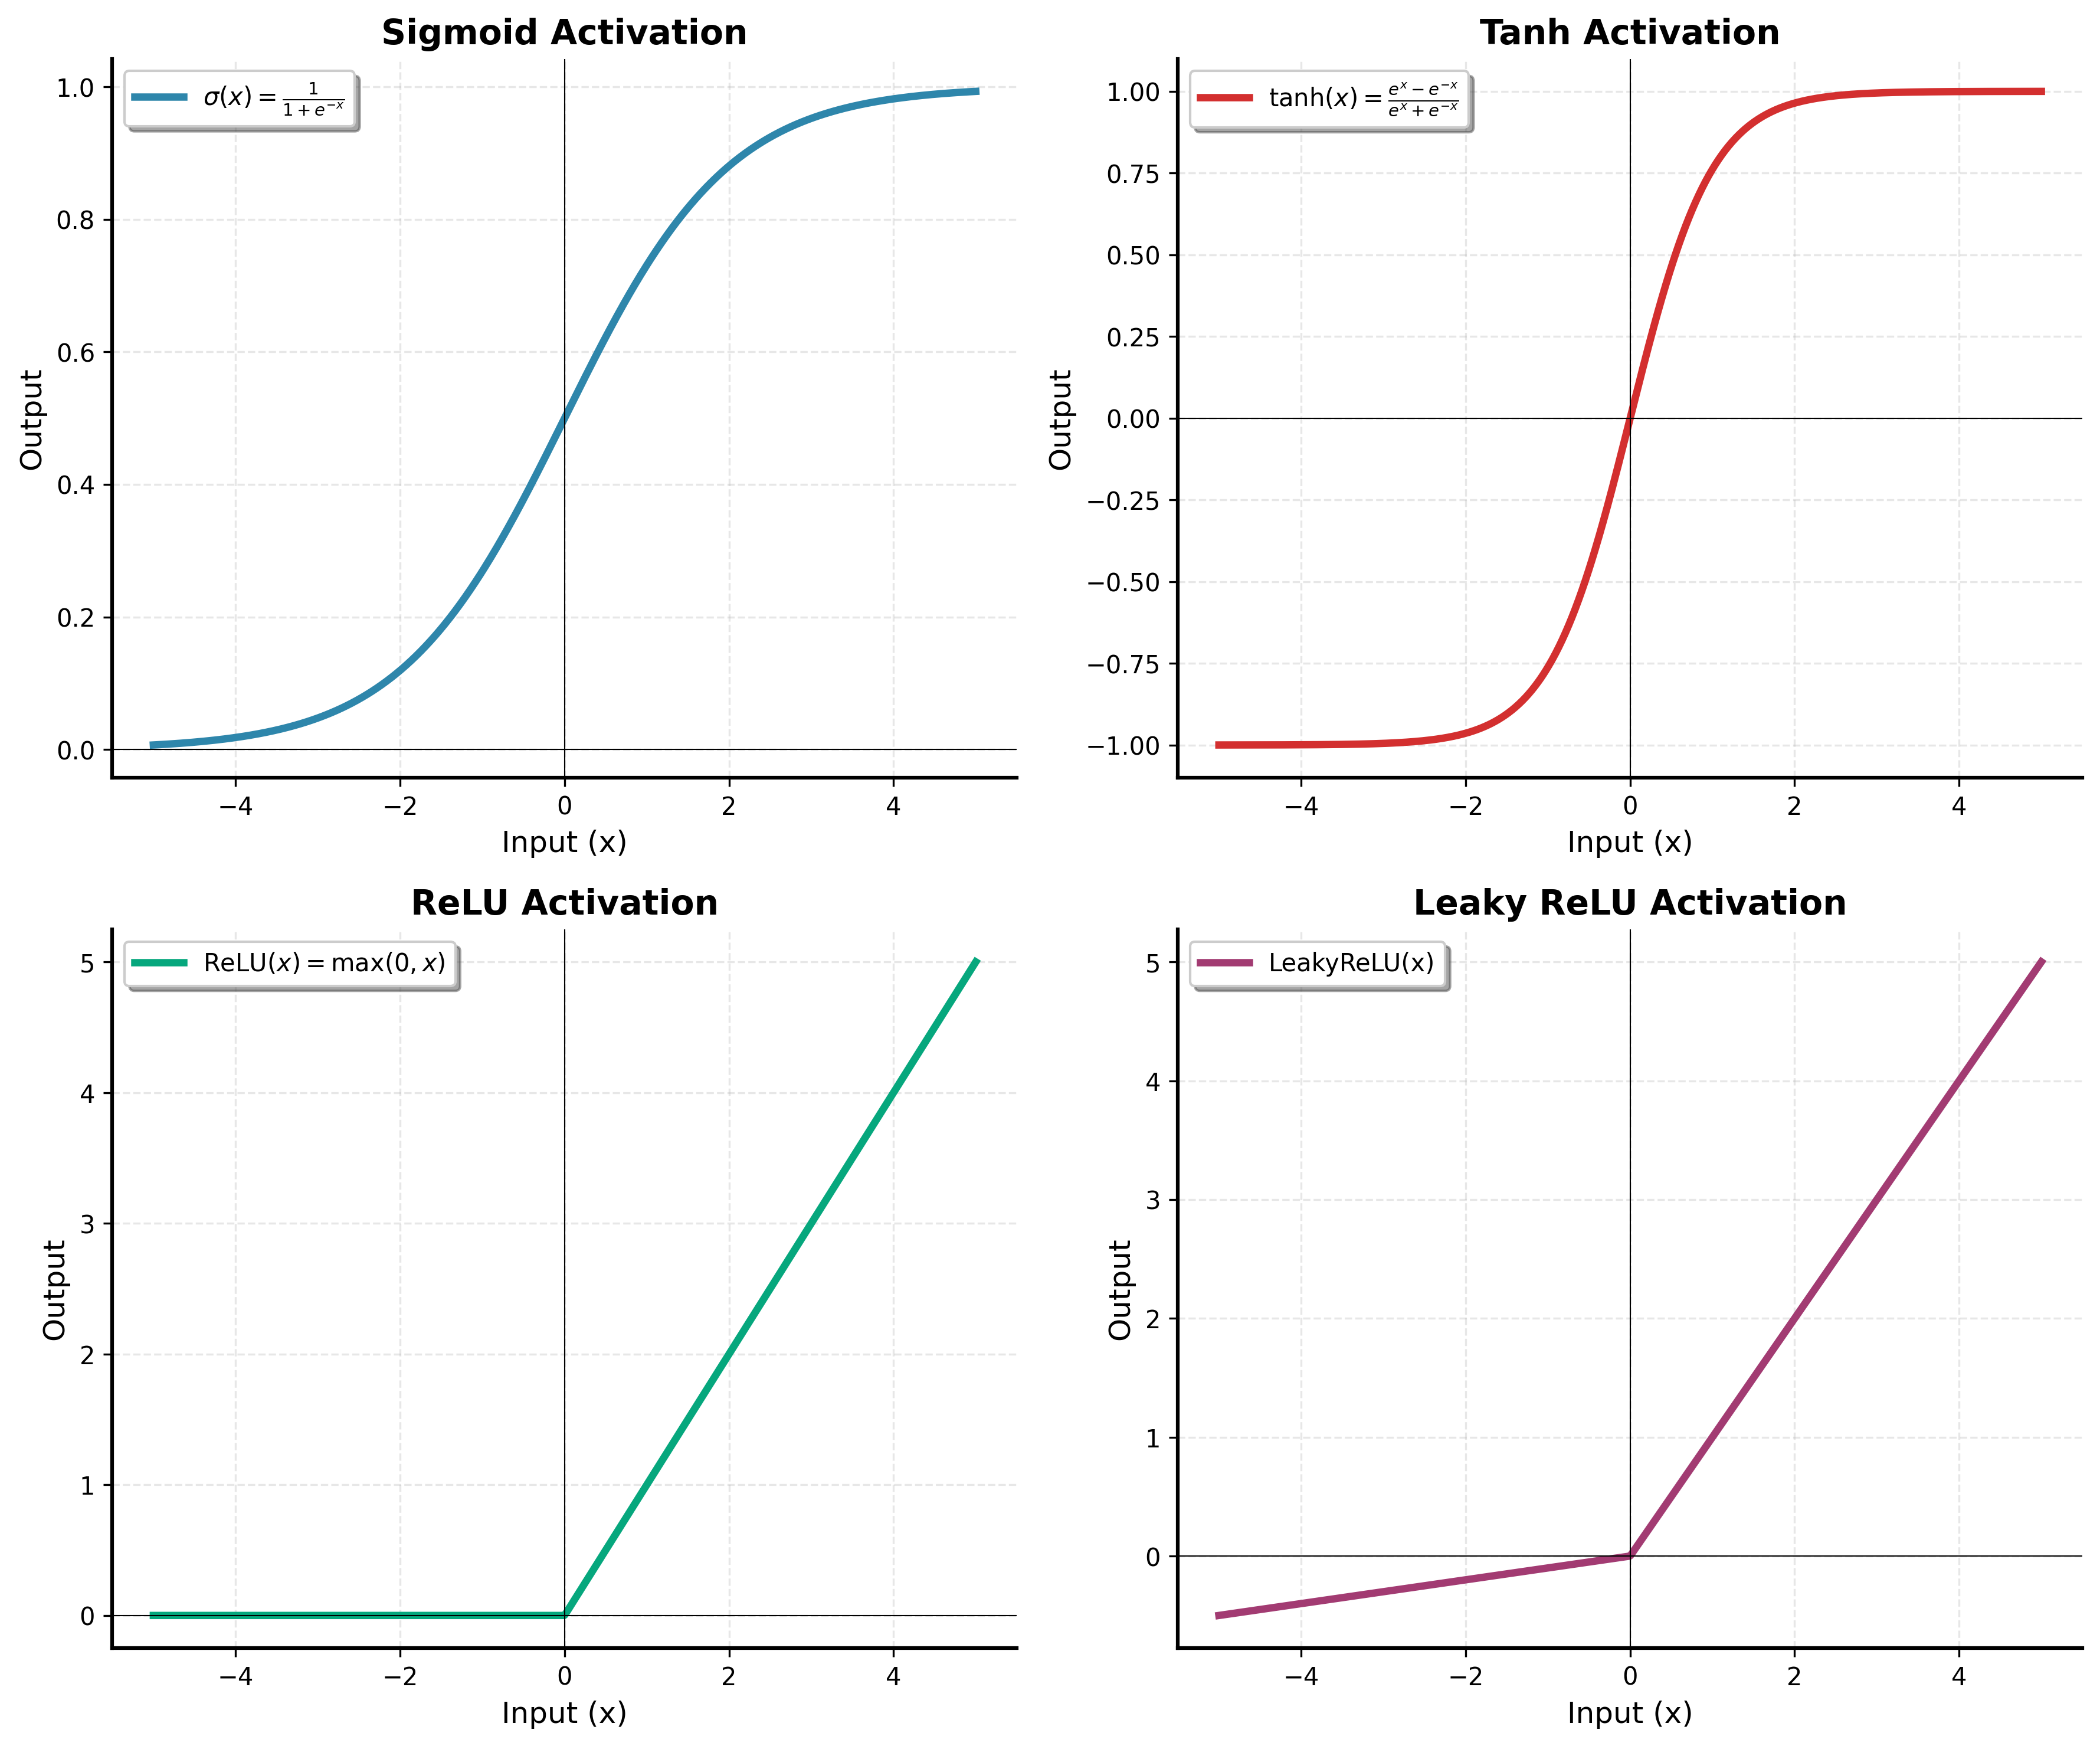
\includegraphics[width=0.7\textwidth]{../figures/activation_functions.png}

\vspace{0.05cm}

\begin{alertblock}{Purpose}
Activation functions introduce \textbf{non-linearity} into the network, enabling it to learn complex patterns.
\end{alertblock}
\end{frame}

\begin{frame}{Activation Functions: Mathematical Properties}
\begin{columns}[t]
\begin{column}{0.48\textwidth}
\begin{block}{Sigmoid Function}
$$\sigma(x) = \frac{1}{1 + e^{-x}}$$

\textbf{Properties:}
\begin{itemize}
\item Range: $(0, 1)$
\item Smooth and differentiable
\item Output interpretable as probability
\end{itemize}

\textbf{Derivative:}
$$\sigma'(x) = \sigma(x)(1 - \sigma(x))$$

\textbf{Issues:} Vanishing gradients for large $|x|$
\end{block}
\end{column}

\begin{column}{0.48\textwidth}
\begin{block}{Hyperbolic Tangent}
$$\tanh(x) = \frac{e^x - e^{-x}}{e^x + e^{-x}}$$

\textbf{Properties:}
\begin{itemize}
\item Range: $(-1, 1)$
\item Zero-centered output
\item Steeper gradients than sigmoid
\end{itemize}

\textbf{Derivative:}
$$\tanh'(x) = 1 - \tanh^2(x)$$

\textbf{Advantage:} Better than sigmoid
\end{block}
\end{column}
\end{columns}
\end{frame}

\begin{frame}{Activation Functions: ReLU Family}
\begin{columns}[t]
\begin{column}{0.48\textwidth}
\begin{block}{ReLU (Rectified Linear Unit)}
$$\text{ReLU}(x) = \max(0, x)$$

\textbf{Advantages:}
\begin{itemize}
\item Computationally efficient
\item No vanishing gradient for $x > 0$
\item Sparse activation
\item Most popular choice
\end{itemize}

\textbf{Derivative:}
$$\text{ReLU}'(x) = \begin{cases}
1 & \text{if } x > 0 \\
0 & \text{if } x \leq 0
\end{cases}$$
\end{block}
\end{column}

\begin{column}{0.48\textwidth}
\begin{block}{Leaky ReLU}
$$\text{LeakyReLU}(x) = \begin{cases}
x & \text{if } x > 0 \\
\alpha x & \text{if } x \leq 0
\end{cases}$$

\textbf{Advantages:}
\begin{itemize}
\item Avoids "dying ReLU" problem
\item Small gradient for negative inputs
\item Typically $\alpha = 0.01$
\end{itemize}

\textbf{Derivative:}
$$\text{LeakyReLU}'(x) = \begin{cases}
1 & \text{if } x > 0 \\
\alpha & \text{if } x \leq 0
\end{cases}$$
\end{block}
\end{column}
\end{columns}
\end{frame}

\begin{frame}{Activation Function Derivatives}
\centering
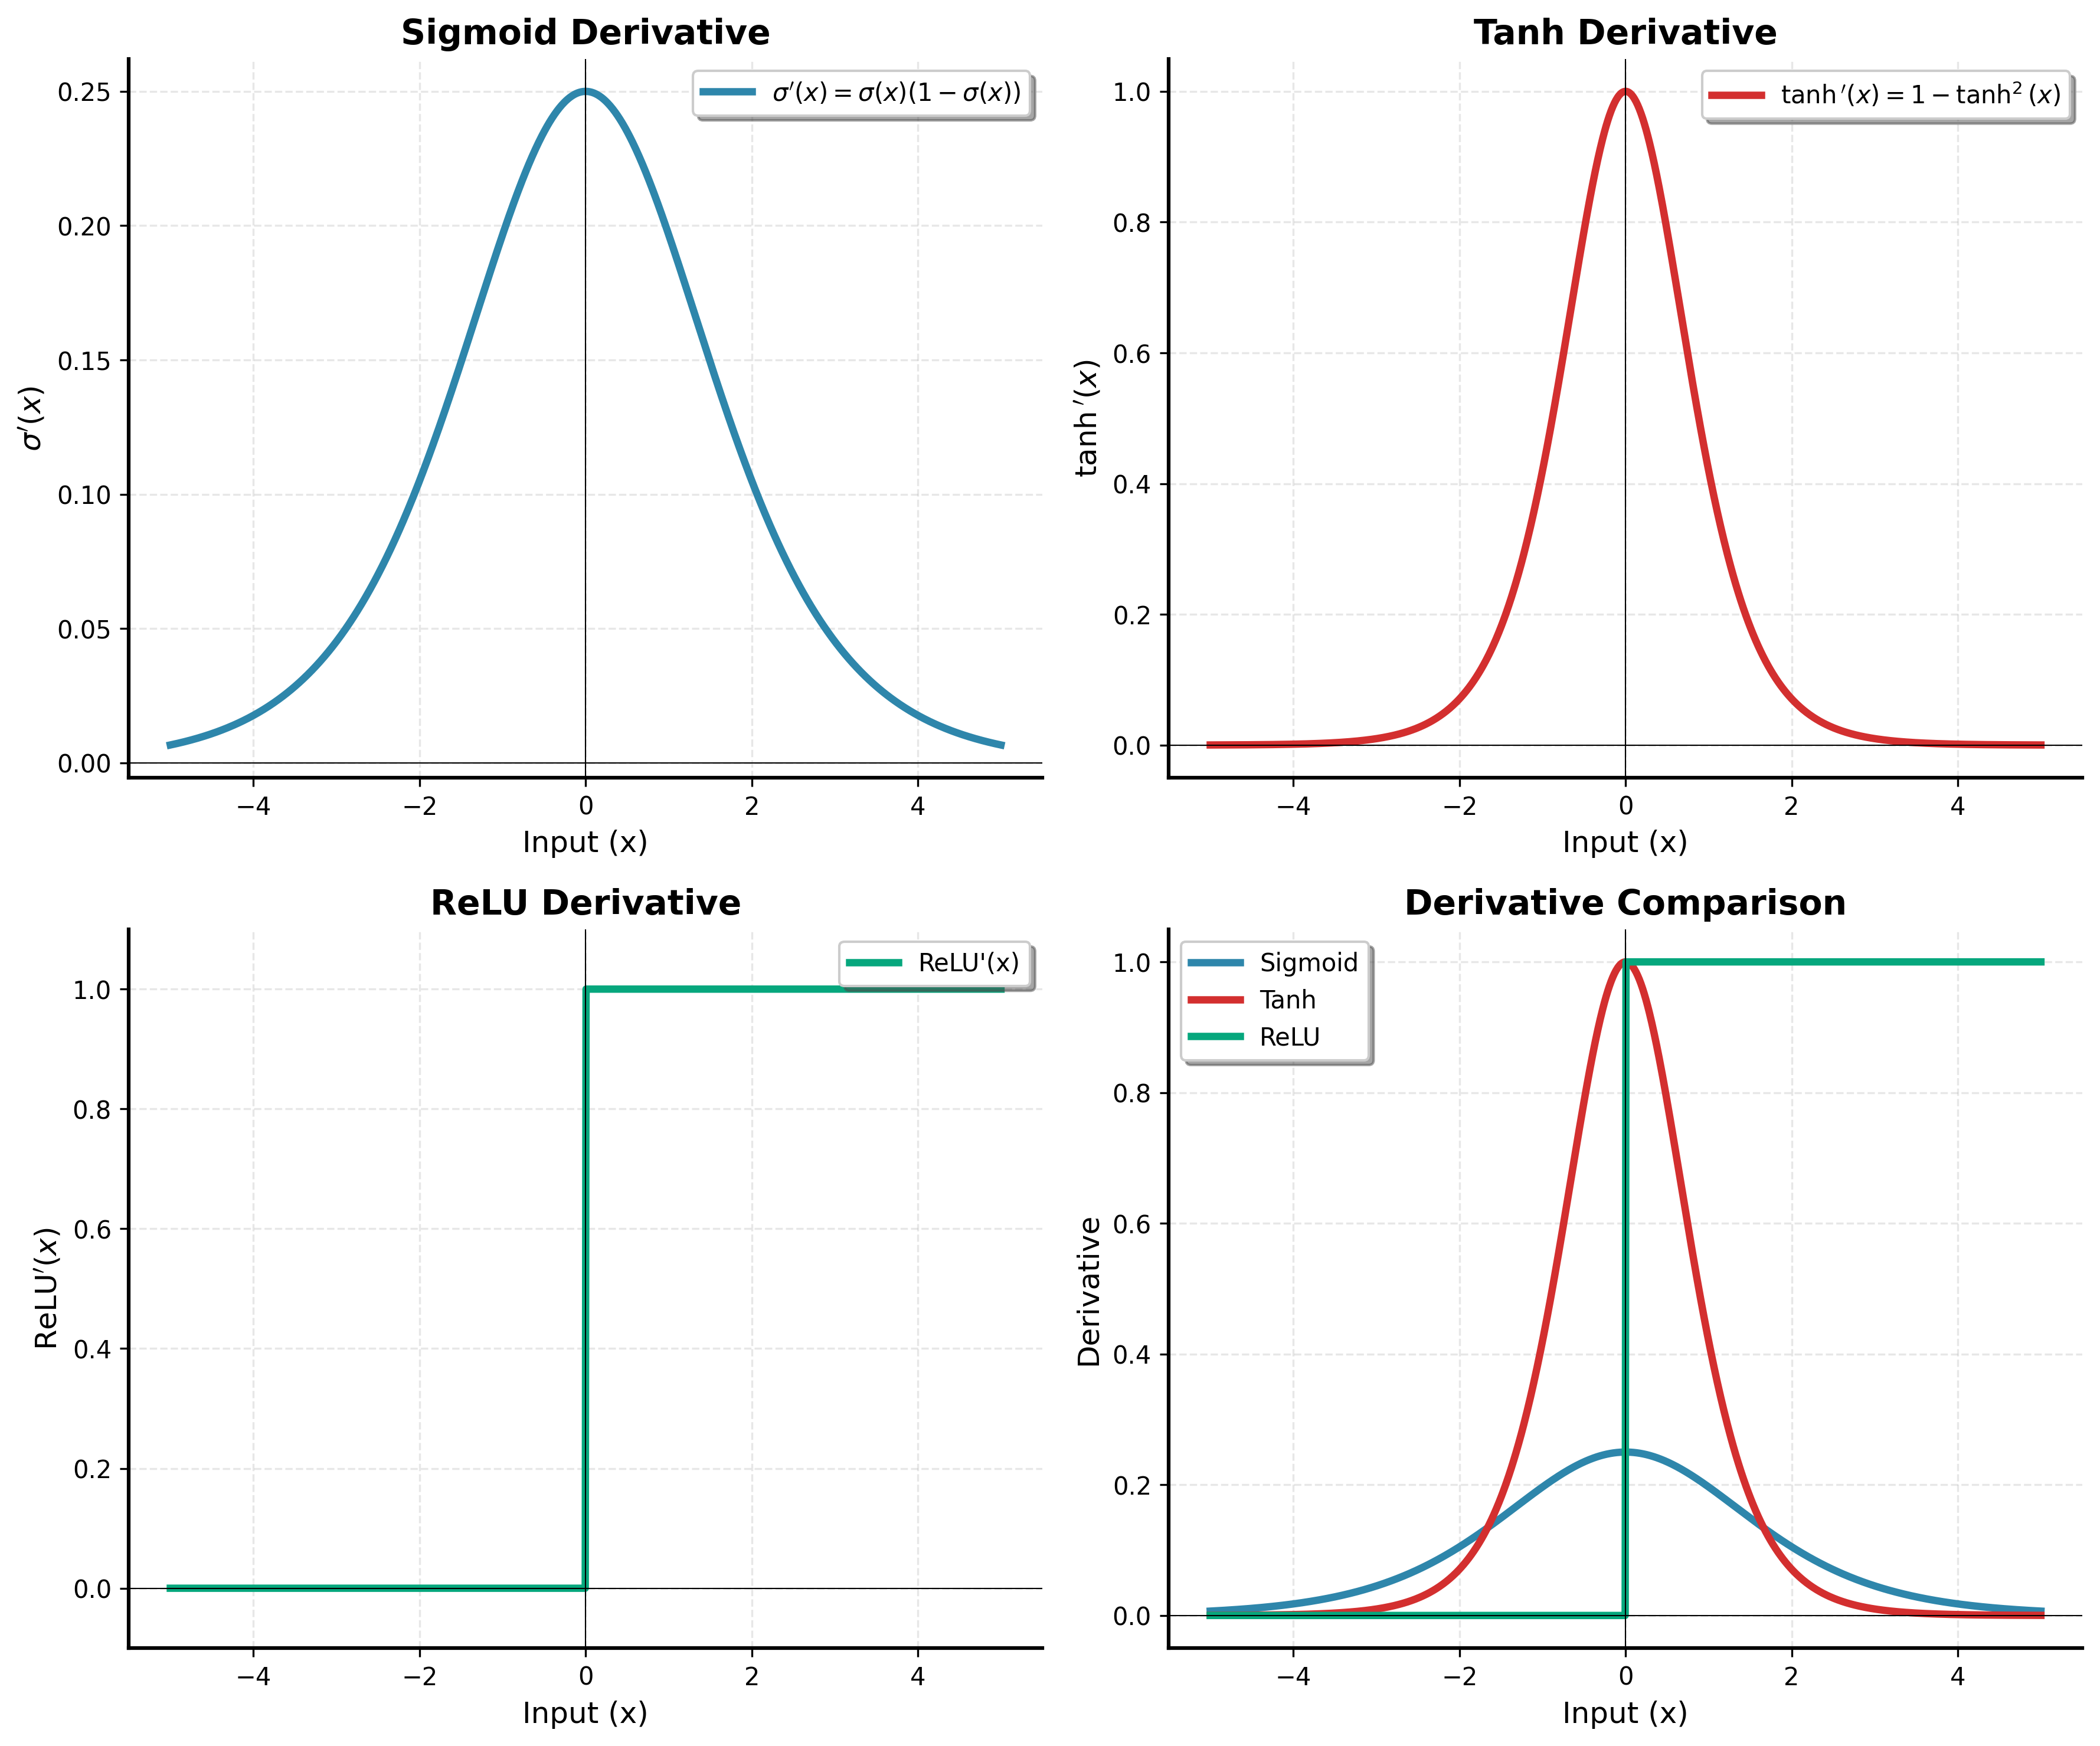
\includegraphics[width=0.7\textwidth]{../figures/activation_derivatives.png}

\vspace{0.05cm}

\begin{alertblock}{Why Derivatives Matter}
Derivatives are crucial for \textbf{backpropagation} - they determine how errors flow backward through the network during training.
\end{alertblock}
\end{frame}

\begin{frame}{Choosing Activation Functions}
\begin{columns}[t]
\begin{column}{0.48\textwidth}
\begin{tipblock}{Guidelines}
\textbf{Hidden Layers:}
\begin{itemize}
\setlength{\itemsep}{1pt}
\item \textbf{ReLU}: Default choice (fast, effective)
\item \textbf{Leaky ReLU}: If dying ReLU is a problem
\item \textbf{Tanh}: For zero-centered data
\item \textbf{Sigmoid}: Avoid (vanishing gradients)
\end{itemize}
\vspace{0.1cm}
\textbf{Output Layer:}
\begin{itemize}
\setlength{\itemsep}{1pt}
\item \textbf{Sigmoid}: Binary classification
\item \textbf{Softmax}: Multi-class classification
\item \textbf{Linear}: Regression
\item \textbf{Tanh}: Regression (bounded output)
\end{itemize}
\end{tipblock}
\end{column}

\begin{column}{0.48\textwidth}
\begin{block}{Common Issues}
\textbf{Vanishing Gradients:}
\begin{itemize}
\setlength{\itemsep}{1pt}
\item Sigmoid/Tanh derivatives $\rightarrow 0$ for large inputs
\item Deep networks suffer from this
\item Solution: ReLU activations
\end{itemize}
\vspace{0.1cm}
\textbf{Dying ReLU:}
\begin{itemize}
\setlength{\itemsep}{1pt}
\item Neurons get stuck at zero output
\item No gradient flows through
\item Solution: Leaky ReLU, initialization
\end{itemize}
\end{block}
\end{column}
\end{columns}

\vspace{0.1cm}

\begin{alertblock}{Best Practice}
\textbf{Start with ReLU} for hidden layers and choose output activation based on your task.
\end{alertblock}
\end{frame}

% ========================================
% Section: Multi-Layer Networks
% ========================================

\section{Multi-Layer Networks \& Architecture}

\begin{frame}{Multi-Layer Neural Network Architecture}
\centering

\begin{tikzpicture}[scale=0.85, every node/.style={scale=0.85}]
    % Input layer - centered vertically
    \foreach \y in {0,1,2,3} {
        \node[input neuron] (I-\y) at (0,{3.5-\y}) {$x_{\y}$};
    }

    % Hidden layer 1 - centered with 5 nodes
    \foreach \y in {0,1,2,3,4} {
        \node[hidden neuron] (H1-\y) at (3,{4-\y}) {};
    }

    % Hidden layer 2 - centered with 3 nodes
    \foreach \y in {0,1,2} {
        \node[hidden neuron] (H2-\y) at (6,{3-\y}) {};
    }

    % Output layer - centered with 2 nodes
    \foreach \y in {0,1} {
        \node[output neuron] (O-\y) at (9,{2-\y}) {$y_{\y}$};
    }

    % Connections input to hidden1
    \foreach \i in {0,1,2,3} {
        \foreach \j in {0,1,2,3,4} {
            \draw[connection, opacity=0.3] (I-\i) -- (H1-\j);
        }
    }

    % Connections hidden1 to hidden2
    \foreach \i in {0,1,2,3,4} {
        \foreach \j in {0,1,2} {
            \draw[connection, opacity=0.3] (H1-\i) -- (H2-\j);
        }
    }

    % Connections hidden2 to output
    \foreach \i in {0,1,2} {
        \foreach \j in {0,1} {
            \draw[connection, opacity=0.3] (H2-\i) -- (O-\j);
        }
    }

    % Layer labels - better positioned
    \node[layer label] at (0,-1.3) {Input};
    \node[layer label] at (3,-1.3) {Hidden 1};
    \node[layer label] at (6,-1.3) {Hidden 2};
    \node[layer label] at (9,-1.3) {Output};

    % Weight matrix labels - positioned above network
    \node[above, font=\small] at (1.5,4.5) {$\mathbf{W}^{(1)}, \mathbf{b}^{(1)}$};
    \node[above, font=\small] at (4.5,4.5) {$\mathbf{W}^{(2)}, \mathbf{b}^{(2)}$};
    \node[above, font=\small] at (7.5,4.5) {$\mathbf{W}^{(3)}, \mathbf{b}^{(3)}$};

    % Forward propagation arrows
    \foreach \x in {1.5,4.5,7.5} {
        \draw[flow arrow] (\x,-0.8) -- (\x+1,-0.8);
    }
    \node[below] at (4.5,-0.8) {\textbf{Forward Propagation}};
\end{tikzpicture}

\vspace{0.3cm}

\begin{alertblock}{Key Components}
\textbf{Layers:} Input → Hidden → Hidden → ... → Output

\textbf{Connections:} Each neuron connects to all neurons in the next layer (fully connected)
\end{alertblock}
\end{frame}

\begin{frame}{Network Architecture: Mathematical Representation}
\textbf{For a network with $L$ layers:}

\begin{align}
\mathbf{a}^{(0)} &= \mathbf{x} \quad \text{(input layer)} \\
\mathbf{z}^{(l)} &= \mathbf{W}^{(l)} \mathbf{a}^{(l-1)} + \mathbf{b}^{(l)} \quad \text{for } l = 1, 2, \ldots, L \\
\mathbf{a}^{(l)} &= \sigma^{(l)}(\mathbf{z}^{(l)}) \quad \text{for } l = 1, 2, \ldots, L \\
\hat{\mathbf{y}} &= \mathbf{a}^{(L)} \quad \text{(output layer)}
\end{align}

where:
\begin{itemize}
\setlength{\itemsep}{2pt}
\item $\mathbf{W}^{(l)} \in \mathbb{R}^{n_l \times n_{l-1}}$: weight matrix for layer $l$
\item $\mathbf{b}^{(l)} \in \mathbb{R}^{n_l}$: bias vector for layer $l$
\item $n_l$: number of neurons in layer $l$
\item $\sigma^{(l)}$: activation function for layer $l$
\end{itemize}
\end{frame}

\begin{frame}{Network Dimensions and Parameters}
\begin{columns}[t]
\begin{column}{0.48\textwidth}
\begin{block}{Matrix Dimensions}
For layer $l$:
\begin{itemize}
\item Input: $\mathbf{a}^{(l-1)}$ has shape $(n_{l-1}, 1)$
\item Weights: $\mathbf{W}^{(l)}$ has shape $(n_l, n_{l-1})$
\item Output: $\mathbf{a}^{(l)}$ has shape $(n_l, 1)$
\end{itemize}

\vspace{0.3cm}

\textbf{Batch Processing:}
\begin{itemize}
\item Input batch: $\mathbf{A}^{(l-1)}$ has shape $(n_{l-1}, m)$
\item Output batch: $\mathbf{A}^{(l)}$ has shape $(n_l, m)$
\item where $m$ is the batch size
\end{itemize}
\end{block}
\end{column}

\begin{column}{0.48\textwidth}
\begin{block}{Parameter Count}
Total parameters:
$$\sum_{l=1}^{L} (n_l \times n_{l-1} + n_l)$$

\textbf{Example:} 784 → 128 → 64 → 10
\begin{align}
&784 \times 128 + 128 \\
&+ 128 \times 64 + 64 \\
&+ 64 \times 10 + 10 \\
&= 109,386 \text{ parameters}
\end{align}

\textbf{Memory scales with:}
\begin{itemize}
\item Network depth
\item Layer width
\item Batch size
\end{itemize}
\end{block}
\end{column}
\end{columns}
\end{frame}

\begin{frame}{Network Design Considerations}
\begin{columns}[t]
\begin{column}{0.48\textwidth}
\begin{block}{Depth vs Width}
\textbf{Deeper Networks:}
\begin{itemize}
\setlength{\itemsep}{2pt}
\item More layers, fewer neurons per layer
\item Better feature hierarchies
\item Can represent more complex functions
\item Risk: vanishing gradients
\end{itemize}

\textbf{Wider Networks:}
\begin{itemize}
\setlength{\itemsep}{2pt}
\item Fewer layers, more neurons per layer
\item More parameters at each level
\item Easier to train
\item Risk: overfitting
\end{itemize}
\end{block}
\end{column}

\begin{column}{0.48\textwidth}
\begin{tipblock}{Architecture Guidelines}
\textbf{Hidden Layer Size:}
\begin{itemize}
\setlength{\itemsep}{2pt}
\item Start with 1-2 hidden layers
\item Size between input and output dimensions
\item Rule of thumb: $\sqrt{n_{input} \times n_{output}}$
\end{itemize}

\textbf{Number of Layers:}
\begin{itemize}
\setlength{\itemsep}{2pt}
\item Simple problems: 1-2 hidden layers
\item Complex problems: 3+ layers
\item Very deep: Requires special techniques
\end{itemize}
\end{tipblock}
\end{column}
\end{columns}

\vspace{0.2cm}

\begin{alertblock}{Rule of Thumb}
Start simple and gradually increase complexity. Use validation performance to guide architecture choices.
\end{alertblock}
\end{frame}

% ========================================
% Section: Forward Propagation
% ========================================

\section{Forward Propagation}

\begin{frame}{Forward Propagation: Information Flow}
\centering

\begin{tikzpicture}[scale=1.0, every node/.style={scale=1.0}]
    % Network structure (simplified 3-layer) - centered vertically
    \node[input neuron] (x1) at (0,2) {$x_1$};
    \node[input neuron] (x2) at (0,1) {$x_2$};
    \node[input neuron] (x3) at (0,0) {$x_3$};

    \node[hidden neuron] (h1) at (3.5,1.5) {$h_1$};
    \node[hidden neuron] (h2) at (3.5,0.5) {$h_2$};

    \node[output neuron] (y) at (7,1) {$y$};

    % Connections with reduced opacity
    \draw[strong connection, opacity=0.25] (x1) -- (h1);
    \draw[strong connection, opacity=0.25] (x1) -- (h2);
    \draw[strong connection, opacity=0.25] (x2) -- (h1);
    \draw[strong connection, opacity=0.25] (x2) -- (h2);
    \draw[strong connection, opacity=0.25] (x3) -- (h1);
    \draw[strong connection, opacity=0.25] (x3) -- (h2);

    \draw[strong connection, opacity=0.25] (h1) -- (y);
    \draw[strong connection, opacity=0.25] (h2) -- (y);

    % Flow arrows and computations - positioned above network
    \node[computation] (z1) at (1.75,2.8) {$\mathbf{z}^{(1)}$};
    \node[activation] (a1) at (1.75,3.6) {$\sigma$};
    \draw[flow arrow] (z1) -- (a1);
    \node[above=0.1cm of a1, font=\small] {$\mathbf{a}^{(1)} = \sigma(\mathbf{z}^{(1)})$};

    \node[computation] (z2) at (5.25,2.8) {$\mathbf{z}^{(2)}$};
    \node[activation] (a2) at (5.25,3.6) {$\sigma$};
    \draw[flow arrow] (z2) -- (a2);
    \node[above=0.1cm of a2, font=\small] {$\mathbf{a}^{(2)} = \sigma(\mathbf{z}^{(2)})$};

    % Mathematical formulation - better positioning
    \node[below, font=\small] at (1.75,-0.8) {$\mathbf{z}^{(1)} = \mathbf{W}^{(1)}\mathbf{x} + \mathbf{b}^{(1)}$};
    \node[below, font=\small] at (5.25,-0.8) {$\mathbf{z}^{(2)} = \mathbf{W}^{(2)}\mathbf{a}^{(1)} + \mathbf{b}^{(2)}$};

    % Layer labels
    \node[layer label] at (0,-1.5) {Input};
    \node[layer label] at (3.5,-1.5) {Hidden};
    \node[layer label] at (7,-1.5) {Output};

    % Forward flow arrows - positioned below labels
    \draw[flow arrow, very thick] (0.8,-1.3) -- (2.7,-1.3);
    \draw[flow arrow, very thick] (4.3,-1.3) -- (6.2,-1.3);
    \node[below, font=\small\bfseries] at (3.5,-1.1) {Forward Propagation};
\end{tikzpicture}

\vspace{0.3cm}

\begin{alertblock}{Forward Pass}
Information flows from \textbf{input to output}, layer by layer, to compute predictions.
\end{alertblock}
\end{frame}

\begin{frame}{Forward Propagation Algorithm}
\textbf{Step-by-step Process:}

\begin{algorithm}[H]
\caption{Forward Propagation}
\begin{algorithmic}[1]
\STATE \textbf{Input:} $\mathbf{x}$, weights $\{\mathbf{W}^{(l)}\}$, biases $\{\mathbf{b}^{(l)}\}$
\STATE Set $\mathbf{a}^{(0)} = \mathbf{x}$
\FOR{$l = 1$ to $L$}
    \STATE Compute pre-activation: $\mathbf{z}^{(l)} = \mathbf{W}^{(l)} \mathbf{a}^{(l-1)} + \mathbf{b}^{(l)}$
    \STATE Apply activation: $\mathbf{a}^{(l)} = \sigma^{(l)}(\mathbf{z}^{(l)})$
\ENDFOR
\STATE \textbf{Output:} $\hat{\mathbf{y}} = \mathbf{a}^{(L)}$
\end{algorithmic}
\end{algorithm}

\vspace{0.3cm}

\begin{columns}[t]
\begin{column}{0.48\textwidth}
\begin{exampleblock}{Vectorized Implementation}
\textbf{For batch processing:}
\begin{align}
\mathbf{Z}^{(l)} &= \mathbf{A}^{(l-1)} \mathbf{W}^{(l)T} + \mathbf{b}^{(l)} \\
\mathbf{A}^{(l)} &= \sigma^{(l)}(\mathbf{Z}^{(l)})
\end{align}

where $\mathbf{A}^{(l)}$ has shape $(m, n_l)$ for $m$ examples.

\textbf{Computational Complexity:} $O(L \cdot N \cdot M)$
where $L$ = layers, $N$ = max neurons/layer, $M$ = batch size
\end{exampleblock}
\end{column}

\begin{column}{0.48\textwidth}
\begin{exampleblock}{Example Calculation}
Network: $2 \rightarrow 3 \rightarrow 1$
Input: $\mathbf{x} = [0.5, 0.8]^T$

\textbf{Layer 1:}
$\mathbf{z}^{(1)} = \mathbf{W}^{(1)} \mathbf{x} + \mathbf{b}^{(1)}$
$\mathbf{a}^{(1)} = \sigma(\mathbf{z}^{(1)})$

\textbf{Layer 2:}
$z^{(2)} = \mathbf{w}^{(2)T} \mathbf{a}^{(1)} + b^{(2)}$
$\hat{y} = \sigma(z^{(2)})$

All intermediate values $\mathbf{z}^{(l)}, \mathbf{a}^{(l)}$ are stored for backpropagation.
\end{exampleblock}
\end{column}
\end{columns}
\end{frame}

\begin{frame}{Forward Propagation: Implementation Details}
\begin{columns}[t]
\begin{column}{0.48\textwidth}
\begin{block}{Memory Considerations}
\textbf{Storage Requirements:}
\begin{itemize}
\setlength{\itemsep}{2pt}
\item Store all activations $\mathbf{a}^{(l)}$
\item Store all pre-activations $\mathbf{z}^{(l)}$
\item Needed for backpropagation
\end{itemize}

\textbf{Memory Usage:}
$$\text{Memory} \propto \sum_{l=0}^{L} n_l \times \text{batch\_size}$$

\textbf{Trade-offs:}
\begin{itemize}
\setlength{\itemsep}{2pt}
\item Larger batches: More memory, better GPU utilization
\item Smaller batches: Less memory, more gradient noise
\end{itemize}
\end{block}
\end{column}

\begin{column}{0.48\textwidth}
\begin{techblock}{Numerical Stability}
\textbf{Common Issues:}
\begin{itemize}
\setlength{\itemsep}{2pt}
\item \textbf{Overflow:} Large intermediate values
\item \textbf{Underflow:} Very small values → 0
\item \textbf{NaN propagation:} Invalid operations
\end{itemize}

\textbf{Solutions:}
\begin{itemize}
\setlength{\itemsep}{2pt}
\item Proper weight initialization
\item Batch normalization
\item Gradient clipping
\item Use stable activation functions (ReLU)
\end{itemize}
\end{techblock}
\end{column}
\end{columns}

\vspace{0.2cm}

\begin{alertblock}{Key Insight}
Forward propagation is computationally straightforward, but proper implementation requires attention to \textbf{memory usage} and \textbf{numerical stability}.
\end{alertblock}
\end{frame}

\begin{frame}{Forward Pass: Handworked Example}
\textbf{Network:} 2 inputs → 2 hidden → 1 output (sigmoid activation)

\begin{columns}[t]
\begin{column}{0.48\textwidth}
\begin{block}{Given}
\textbf{Input:} $\mathbf{x} = \begin{bmatrix} 0.5 \\ 0.8 \end{bmatrix}$

\textbf{Weights \& Biases:}
$$\mathbf{W}^{(1)} = \begin{bmatrix} 0.2 & 0.4 \\ 0.3 & 0.1 \end{bmatrix}, \quad \mathbf{b}^{(1)} = \begin{bmatrix} 0.1 \\ 0.2 \end{bmatrix}$$

$$\mathbf{W}^{(2)} = \begin{bmatrix} 0.6 & 0.5 \end{bmatrix}, \quad b^{(2)} = 0.3$$

\textbf{Activation:} $\sigma(z) = \frac{1}{1 + e^{-z}}$
\end{block}
\end{column}

\begin{column}{0.48\textwidth}
\begin{block}{Step 1: Hidden Layer}
$$\mathbf{z}^{(1)} = \mathbf{W}^{(1)} \mathbf{x} + \mathbf{b}^{(1)}$$

$$= \begin{bmatrix} 0.2 & 0.4 \\ 0.3 & 0.1 \end{bmatrix} \begin{bmatrix} 0.5 \\ 0.8 \end{bmatrix} + \begin{bmatrix} 0.1 \\ 0.2 \end{bmatrix}$$

$$= \begin{bmatrix} 0.2(0.5) + 0.4(0.8) \\ 0.3(0.5) + 0.1(0.8) \end{bmatrix} + \begin{bmatrix} 0.1 \\ 0.2 \end{bmatrix}$$

$$= \begin{bmatrix} 0.1 + 0.32 \\ 0.15 + 0.08 \end{bmatrix} + \begin{bmatrix} 0.1 \\ 0.2 \end{bmatrix} = \begin{bmatrix} 0.52 \\ 0.43 \end{bmatrix}$$
\end{block}
\end{column}
\end{columns}
\end{frame}

\begin{frame}{Forward Pass: Handworked Example (continued)}
\begin{columns}[t]
\begin{column}{0.48\textwidth}
\begin{block}{Step 2: Hidden Activations}
$$\mathbf{a}^{(1)} = \sigma(\mathbf{z}^{(1)}) = \sigma\left(\begin{bmatrix} 0.52 \\ 0.43 \end{bmatrix}\right)$$

$$a_1^{(1)} = \sigma(0.52) = \frac{1}{1 + e^{-0.52}} = \frac{1}{1 + 0.595} = 0.627$$

$$a_2^{(1)} = \sigma(0.43) = \frac{1}{1 + e^{-0.43}} = \frac{1}{1 + 0.651} = 0.606$$

$$\mathbf{a}^{(1)} = \begin{bmatrix} 0.627 \\ 0.606 \end{bmatrix}$$
\end{block}
\end{column}

\begin{column}{0.48\textwidth}
\begin{block}{Step 3: Output Layer}
$$z^{(2)} = \mathbf{W}^{(2)} \mathbf{a}^{(1)} + b^{(2)}$$

$$= \begin{bmatrix} 0.6 & 0.5 \end{bmatrix} \begin{bmatrix} 0.627 \\ 0.606 \end{bmatrix} + 0.3$$

$$= 0.6(0.627) + 0.5(0.606) + 0.3$$

$$= 0.376 + 0.303 + 0.3 = 0.979$$

\textbf{Final Output:}
$$\hat{y} = \sigma(0.979) = \frac{1}{1 + e^{-0.979}} = 0.727$$
\end{block}
\end{column}
\end{columns}

\vspace{0.3cm}

\begin{alertblock}{Summary}
Input $[0.5, 0.8]$ → Hidden $[0.627, 0.606]$ → Output $0.727$
\end{alertblock}
\end{frame}

% ========================================
% Section: Backpropagation
% ========================================

\section{Backpropagation Algorithm}

\begin{frame}{Backpropagation: Error Flow}
\centering

\begin{tikzpicture}[scale=1.0, every node/.style={scale=1.0}]
    % Network structure (same as forward, but show backward flow)
    \node[input neuron] (x1) at (0,2) {$x_1$};
    \node[input neuron] (x2) at (0,1) {$x_2$};
    \node[input neuron] (x3) at (0,0) {$x_3$};

    \node[hidden neuron] (h1) at (3.5,1.5) {$h_1$};
    \node[hidden neuron] (h2) at (3.5,0.5) {$h_2$};

    \node[output neuron] (y) at (7,1) {$y$};

    % Forward connections (lighter)
    \draw[weak connection, opacity=0.15] (x1) -- (h1);
    \draw[weak connection, opacity=0.15] (x1) -- (h2);
    \draw[weak connection, opacity=0.15] (x2) -- (h1);
    \draw[weak connection, opacity=0.15] (x2) -- (h2);
    \draw[weak connection, opacity=0.15] (x3) -- (h1);
    \draw[weak connection, opacity=0.15] (x3) -- (h2);
    \draw[weak connection, opacity=0.15] (h1) -- (y);
    \draw[weak connection, opacity=0.15] (h2) -- (y);

    % Error/gradient flow (backward arrows) - positioned below
    \draw[error arrow, very thick] (6.2,-1.3) -- (4.3,-1.3);
    \draw[error arrow, very thick] (2.7,-1.3) -- (0.8,-1.3);
    \node[below, font=\small\bfseries] at (3.5,-1.1) {Error Backpropagation};

    % Loss function
    \node[function box] (loss) at (8.2,1) {$L$};
    \draw[error arrow] (y) -- (loss);
    \node[right=0.05cm of loss, font=\small] {Loss};

    % Gradient computations - positioned above network
    \node[computation] (grad2) at (5.25,2.8) {$\boldsymbol{\delta}^{(2)}$};
    \node[computation] (grad1) at (1.75,2.8) {$\boldsymbol{\delta}^{(1)}$};

    % Chain rule arrows
    \draw[gradient arrow] (loss) to[bend left=20] (grad2);
    \draw[gradient arrow] (grad2) to[bend left=20] (grad1);

    % Mathematical formulation - better positioning
    \node[below, font=\small] at (1.75,-0.8) {$\frac{\partial L}{\partial \mathbf{W}^{(1)}} = \boldsymbol{\delta}^{(1)} \mathbf{x}^T$};
    \node[below, font=\small] at (5.25,-0.8) {$\frac{\partial L}{\partial \mathbf{W}^{(2)}} = \boldsymbol{\delta}^{(2)} (\mathbf{a}^{(1)})^T$};

    % Layer labels
    \node[layer label] at (0,-1.5) {Input};
    \node[layer label] at (3.5,-1.5) {Hidden};
    \node[layer label] at (7,-1.5) {Output};

    % Gradient flow labels - above network
    \node[above=0.1cm of grad1, font=\scriptsize] {$\boldsymbol{\delta}^{(1)} = (\mathbf{W}^{(2)})^T \boldsymbol{\delta}^{(2)} \odot \sigma'(\mathbf{z}^{(1)})$};
    \node[above=0.1cm of grad2, font=\scriptsize] {$\boldsymbol{\delta}^{(2)} = \frac{\partial L}{\partial \mathbf{a}^{(2)}} \odot \sigma'(\mathbf{z}^{(2)})$};
\end{tikzpicture}

\vspace{0.3cm}

\begin{alertblock}{Backpropagation}
Efficient algorithm to compute gradients by propagating errors \textbf{backward} through the network using the \textbf{chain rule}.
\end{alertblock}
\end{frame}

\begin{frame}{Mathematical Foundation: Chain Rule}
\textbf{Goal:} Compute $\frac{\partial L}{\partial \mathbf{W}^{(l)}}$ and $\frac{\partial L}{\partial \mathbf{b}^{(l)}}$ for all layers

\vspace{0.05cm}

\textbf{Chain Rule Application:}
\begin{align}
\frac{\partial L}{\partial \mathbf{W}^{(l)}} &= \frac{\partial L}{\partial \mathbf{z}^{(l)}} \frac{\partial \mathbf{z}^{(l)}}{\partial \mathbf{W}^{(l)}} \\
\frac{\partial L}{\partial \mathbf{b}^{(l)}} &= \frac{\partial L}{\partial \mathbf{z}^{(l)}} \frac{\partial \mathbf{z}^{(l)}}{\partial \mathbf{b}^{(l)}} \\
\frac{\partial L}{\partial \mathbf{a}^{(l-1)}} &= \frac{\partial L}{\partial \mathbf{z}^{(l)}} \frac{\partial \mathbf{z}^{(l)}}{\partial \mathbf{a}^{(l-1)}}
\end{align}

\vspace{0.05cm}

\textbf{Key Insight:} Define error terms $\boldsymbol{\delta}^{(l)} = \frac{\partial L}{\partial \mathbf{z}^{(l)}}$

\begin{columns}[t]
\begin{column}{0.48\textwidth}
\begin{block}{Gradient Computations}
\begin{align}
\frac{\partial L}{\partial \mathbf{W}^{(l)}} &= \boldsymbol{\delta}^{(l)} (\mathbf{a}^{(l-1)})^T \\
\frac{\partial L}{\partial \mathbf{b}^{(l)}} &= \boldsymbol{\delta}^{(l)} \\
\boldsymbol{\delta}^{(l-1)} &= (\mathbf{W}^{(l)})^T \boldsymbol{\delta}^{(l)} \odot \sigma'(\mathbf{z}^{(l-1)})
\end{align}
\end{block}
\end{column}

\begin{column}{0.48\textwidth}
\begin{block}{Output Layer}
For output layer $L$:
$$\boldsymbol{\delta}^{(L)} = \frac{\partial L}{\partial \mathbf{a}^{(L)}} \odot \sigma'(\mathbf{z}^{(L)})$$

Common case (MSE + sigmoid):
$$\boldsymbol{\delta}^{(L)} = (\mathbf{a}^{(L)} - \mathbf{y}) \odot \mathbf{a}^{(L)} \odot (1 - \mathbf{a}^{(L)})$$
\end{block}
\end{column}
\end{columns}

where $\odot$ denotes element-wise multiplication.
\end{frame}

\begin{frame}{Backpropagation Algorithm}
\begin{algorithm}[H]
\caption{Backpropagation}
\begin{algorithmic}[1]
\STATE \textbf{Input:} Training example $(\mathbf{x}, \mathbf{y})$, network weights
\STATE \textbf{Forward Pass:} Compute all $\mathbf{a}^{(l)}$ and $\mathbf{z}^{(l)}$ (store them!)
\STATE \textbf{Compute Output Error:} $\boldsymbol{\delta}^{(L)} = \frac{\partial L}{\partial \mathbf{a}^{(L)}} \odot \sigma'(\mathbf{z}^{(L)})$
\FOR{$l = L-1$ down to $1$}
    \STATE \textbf{Propagate Error:} $\boldsymbol{\delta}^{(l)} = (\mathbf{W}^{(l+1)})^T \boldsymbol{\delta}^{(l+1)} \odot \sigma'(\mathbf{z}^{(l)})$
\ENDFOR
\FOR{$l = 1$ to $L$}
    \STATE \textbf{Compute Gradients:}
    \STATE $\frac{\partial L}{\partial \mathbf{W}^{(l)}} = \boldsymbol{\delta}^{(l)} (\mathbf{a}^{(l-1)})^T$
    \STATE $\frac{\partial L}{\partial \mathbf{b}^{(l)}} = \boldsymbol{\delta}^{(l)}$
\ENDFOR
\end{algorithmic}
\end{algorithm}

\vspace{0.1cm}

\begin{columns}[t]
\begin{column}{0.48\textwidth}
\begin{block}{Computational Complexity}
\textbf{Time:} $O(\text{number of weights})$
\begin{itemize}
\setlength{\itemsep}{0pt}
\item Same order as forward pass
\item Very efficient vs numerical gradients
\end{itemize}
\textbf{Space:} $O(\text{network size})$
\begin{itemize}
\setlength{\itemsep}{0pt}
\item Must store all activations
\item Memory scales with depth
\end{itemize}
\end{block}
\end{column}

\begin{column}{0.48\textwidth}
\begin{block}{Why Backpropagation Works}
\begin{itemize}
\setlength{\itemsep}{0pt}
\item \textbf{Efficiency:} Reuses computations via chain rule
\item \textbf{Automatic:} No manual gradient derivation
\item \textbf{Exact:} Computes exact gradients
\item \textbf{General:} Works for any differentiable network
\end{itemize}
\textbf{Historical Impact:}
\begin{itemize}
\setlength{\itemsep}{0pt}
\item Rumelhart, Hinton, Williams (1986)
\item Made deep learning practical
\end{itemize}
\end{block}
\end{column}
\end{columns}
\end{frame}

\begin{frame}{Computational Graph Perspective}
\centering

\begin{tikzpicture}[scale=0.9, every node/.style={scale=0.9}]
    % Input nodes - better vertical alignment
    \node[input neuron] (x) at (0,1.8) {$x$};
    \node[input neuron] (w) at (0,0.2) {$w$};

    % Operation nodes (rectangles for operations) - aligned at y=1
    \node[function box] (mul) at (2.5,1) {$\times$};
    \node[function box] (add) at (5,1) {$+$};
    \node[function box] (sig) at (7.5,1) {$\sigma$};

    % Intermediate results - positioned above operations
    \node[computation] (z1) at (2.5,2.2) {$z_1$};
    \node[computation] (z2) at (5,2.2) {$z_2$};
    \node[output neuron] (y) at (10,1) {$y$};

    % Bias - positioned below mul operation
    \node[bias neuron] (b) at (2.5,-0.6) {$b$};

    % Forward edges
    \draw[flow arrow] (x) -- (mul);
    \draw[flow arrow] (w) -- (mul);
    \draw[flow arrow] (mul) -- (add);
    \draw[flow arrow] (b) -- (add);
    \draw[flow arrow] (add) -- (sig);
    \draw[flow arrow] (sig) -- (y);

    % Intermediate value labels - better positioning
    \draw[connection] (mul) -- (z1) node[midway, right, font=\tiny] {$wx$};
    \draw[connection] (add) -- (z2) node[midway, right, font=\tiny] {$wx + b$};

    % Loss function
    \node[function box] (loss) at (12,1) {$L$};
    \draw[error arrow] (y) -- (loss);

    % Backward gradients (dashed red arrows)
    \draw[gradient arrow] (loss) to[bend left=12] (sig);
    \draw[gradient arrow] (sig) to[bend left=12] (add);
    \draw[gradient arrow] (add) to[bend left=12] (mul);
    \draw[gradient arrow] (add) to[bend right=12] (b);
    \draw[gradient arrow] (mul) to[bend left=12] (x);
    \draw[gradient arrow] (mul) to[bend right=12] (w);

    % Gradient labels - cleaner positioning
    \node[above, font=\tiny] at (11,1.4) {$\frac{\partial L}{\partial y}$};
    \node[above, font=\tiny] at (8.75,1.4) {$\frac{\partial L}{\partial z_2}$};
    \node[above, font=\tiny] at (6.25,1.4) {$\frac{\partial L}{\partial z_1}$};
    \node[left, font=\tiny] at (1.3,0.6) {$\frac{\partial L}{\partial w}$};
    \node[right, font=\tiny] at (3.2,-0.4) {$\frac{\partial L}{\partial b}$};

    % Mathematical operations - positioned below
    \node[below, font=\small] at (2.5,-1.2) {$z_1 = w \cdot x$};
    \node[below, font=\small] at (5,-1.2) {$z_2 = z_1 + b$};
    \node[below, font=\small] at (7.5,-1.2) {$y = \sigma(z_2)$};
\end{tikzpicture}

\vspace{0.1cm}

\begin{alertblock}{Modern View}
Backpropagation is \textbf{automatic differentiation} applied to computational graphs. Modern frameworks (TensorFlow, PyTorch) build these graphs automatically.
\end{alertblock}
\end{frame}

\begin{frame}{4-Layer Neural Network: Differential Equation Derivation}
\textbf{Network Structure:} Input → Hidden1 → Hidden2 → Hidden3 → Output

\textbf{Forward Pass Equations:}
\begin{align}
\mathbf{a}^{(0)} &= \mathbf{x} \quad \text{(input)} \\
\mathbf{z}^{(1)} &= \mathbf{W}^{(1)} \mathbf{a}^{(0)} + \mathbf{b}^{(1)}, \quad \mathbf{a}^{(1)} = \sigma(\mathbf{z}^{(1)}) \\
\mathbf{z}^{(2)} &= \mathbf{W}^{(2)} \mathbf{a}^{(1)} + \mathbf{b}^{(2)}, \quad \mathbf{a}^{(2)} = \sigma(\mathbf{z}^{(2)}) \\
\mathbf{z}^{(3)} &= \mathbf{W}^{(3)} \mathbf{a}^{(2)} + \mathbf{b}^{(3)}, \quad \mathbf{a}^{(3)} = \sigma(\mathbf{z}^{(3)}) \\
\mathbf{z}^{(4)} &= \mathbf{W}^{(4)} \mathbf{a}^{(3)} + \mathbf{b}^{(4)}, \quad \mathbf{a}^{(4)} = \sigma(\mathbf{z}^{(4)}) \quad \text{(output)}
\end{align}

\textbf{Loss Function:} $L = \frac{1}{2}||\mathbf{a}^{(4)} - \mathbf{y}||^2$

\vspace{0.3cm}

\begin{columns}[t]
\begin{column}{0.48\textwidth}
\begin{block}{Output Layer Error}
Starting from the output layer:
\begin{align}
\boldsymbol{\delta}^{(4)} &= \frac{\partial L}{\partial \mathbf{z}^{(4)}} \\
&= \frac{\partial L}{\partial \mathbf{a}^{(4)}} \odot \frac{\partial \mathbf{a}^{(4)}}{\partial \mathbf{z}^{(4)}} \\
&= (\mathbf{a}^{(4)} - \mathbf{y}) \odot \sigma'(\mathbf{z}^{(4)})
\end{align}
\end{block}
\end{column}

\begin{column}{0.48\textwidth}
\begin{block}{Chain Rule Application}
For hidden layers ($l = 3, 2, 1$):
\begin{align}
\boldsymbol{\delta}^{(l)} &= \frac{\partial L}{\partial \mathbf{z}^{(l)}} \\
&= \frac{\partial L}{\partial \mathbf{z}^{(l+1)}} \frac{\partial \mathbf{z}^{(l+1)}}{\partial \mathbf{a}^{(l)}} \frac{\partial \mathbf{a}^{(l)}}{\partial \mathbf{z}^{(l)}} \\
&= (\mathbf{W}^{(l+1)})^T \boldsymbol{\delta}^{(l+1)} \odot \sigma'(\mathbf{z}^{(l)})
\end{align}
\end{block}
\end{column}
\end{columns}
\end{frame}

\begin{frame}{4-Layer Network: Complete Backpropagation Derivation}
\textbf{Step-by-Step Gradient Computation:}

\begin{columns}[t]
\begin{column}{0.48\textwidth}
\begin{block}{Error Propagation}
\textbf{Layer 4 (Output):}
$$\boldsymbol{\delta}^{(4)} = (\mathbf{a}^{(4)} - \mathbf{y}) \odot \sigma'(\mathbf{z}^{(4)})$$

\textbf{Layer 3:}
$$\boldsymbol{\delta}^{(3)} = (\mathbf{W}^{(4)})^T \boldsymbol{\delta}^{(4)} \odot \sigma'(\mathbf{z}^{(3)})$$

\textbf{Layer 2:}
$$\boldsymbol{\delta}^{(2)} = (\mathbf{W}^{(3)})^T \boldsymbol{\delta}^{(3)} \odot \sigma'(\mathbf{z}^{(2)})$$

\textbf{Layer 1:}
$$\boldsymbol{\delta}^{(1)} = (\mathbf{W}^{(2)})^T \boldsymbol{\delta}^{(2)} \odot \sigma'(\mathbf{z}^{(1)})$$
\end{block}
\end{column}

\begin{column}{0.48\textwidth}
\begin{block}{Weight and Bias Gradients}
For each layer $l = 1, 2, 3, 4$:

\textbf{Weight Gradients:}
$$\frac{\partial L}{\partial \mathbf{W}^{(l)}} = \boldsymbol{\delta}^{(l)} (\mathbf{a}^{(l-1)})^T$$

\textbf{Bias Gradients:}
$$\frac{\partial L}{\partial \mathbf{b}^{(l)}} = \boldsymbol{\delta}^{(l)}$$

\vspace{0.2cm}

\textbf{Update Rules:}
\begin{align}
\mathbf{W}^{(l)} &:= \mathbf{W}^{(l)} - \alpha \frac{\partial L}{\partial \mathbf{W}^{(l)}} \\
\mathbf{b}^{(l)} &:= \mathbf{b}^{(l)} - \alpha \frac{\partial L}{\partial \mathbf{b}^{(l)}}
\end{align}
\end{block}
\end{column}
\end{columns}

\begin{alertblock}{Key Insight}
The error \textbf{flows backward} through the network, with each layer's error depending on the next layer's error multiplied by the transpose of the connecting weights.
\end{alertblock}
\end{frame}

\begin{frame}{Gradient Descent Optimization}
\centering
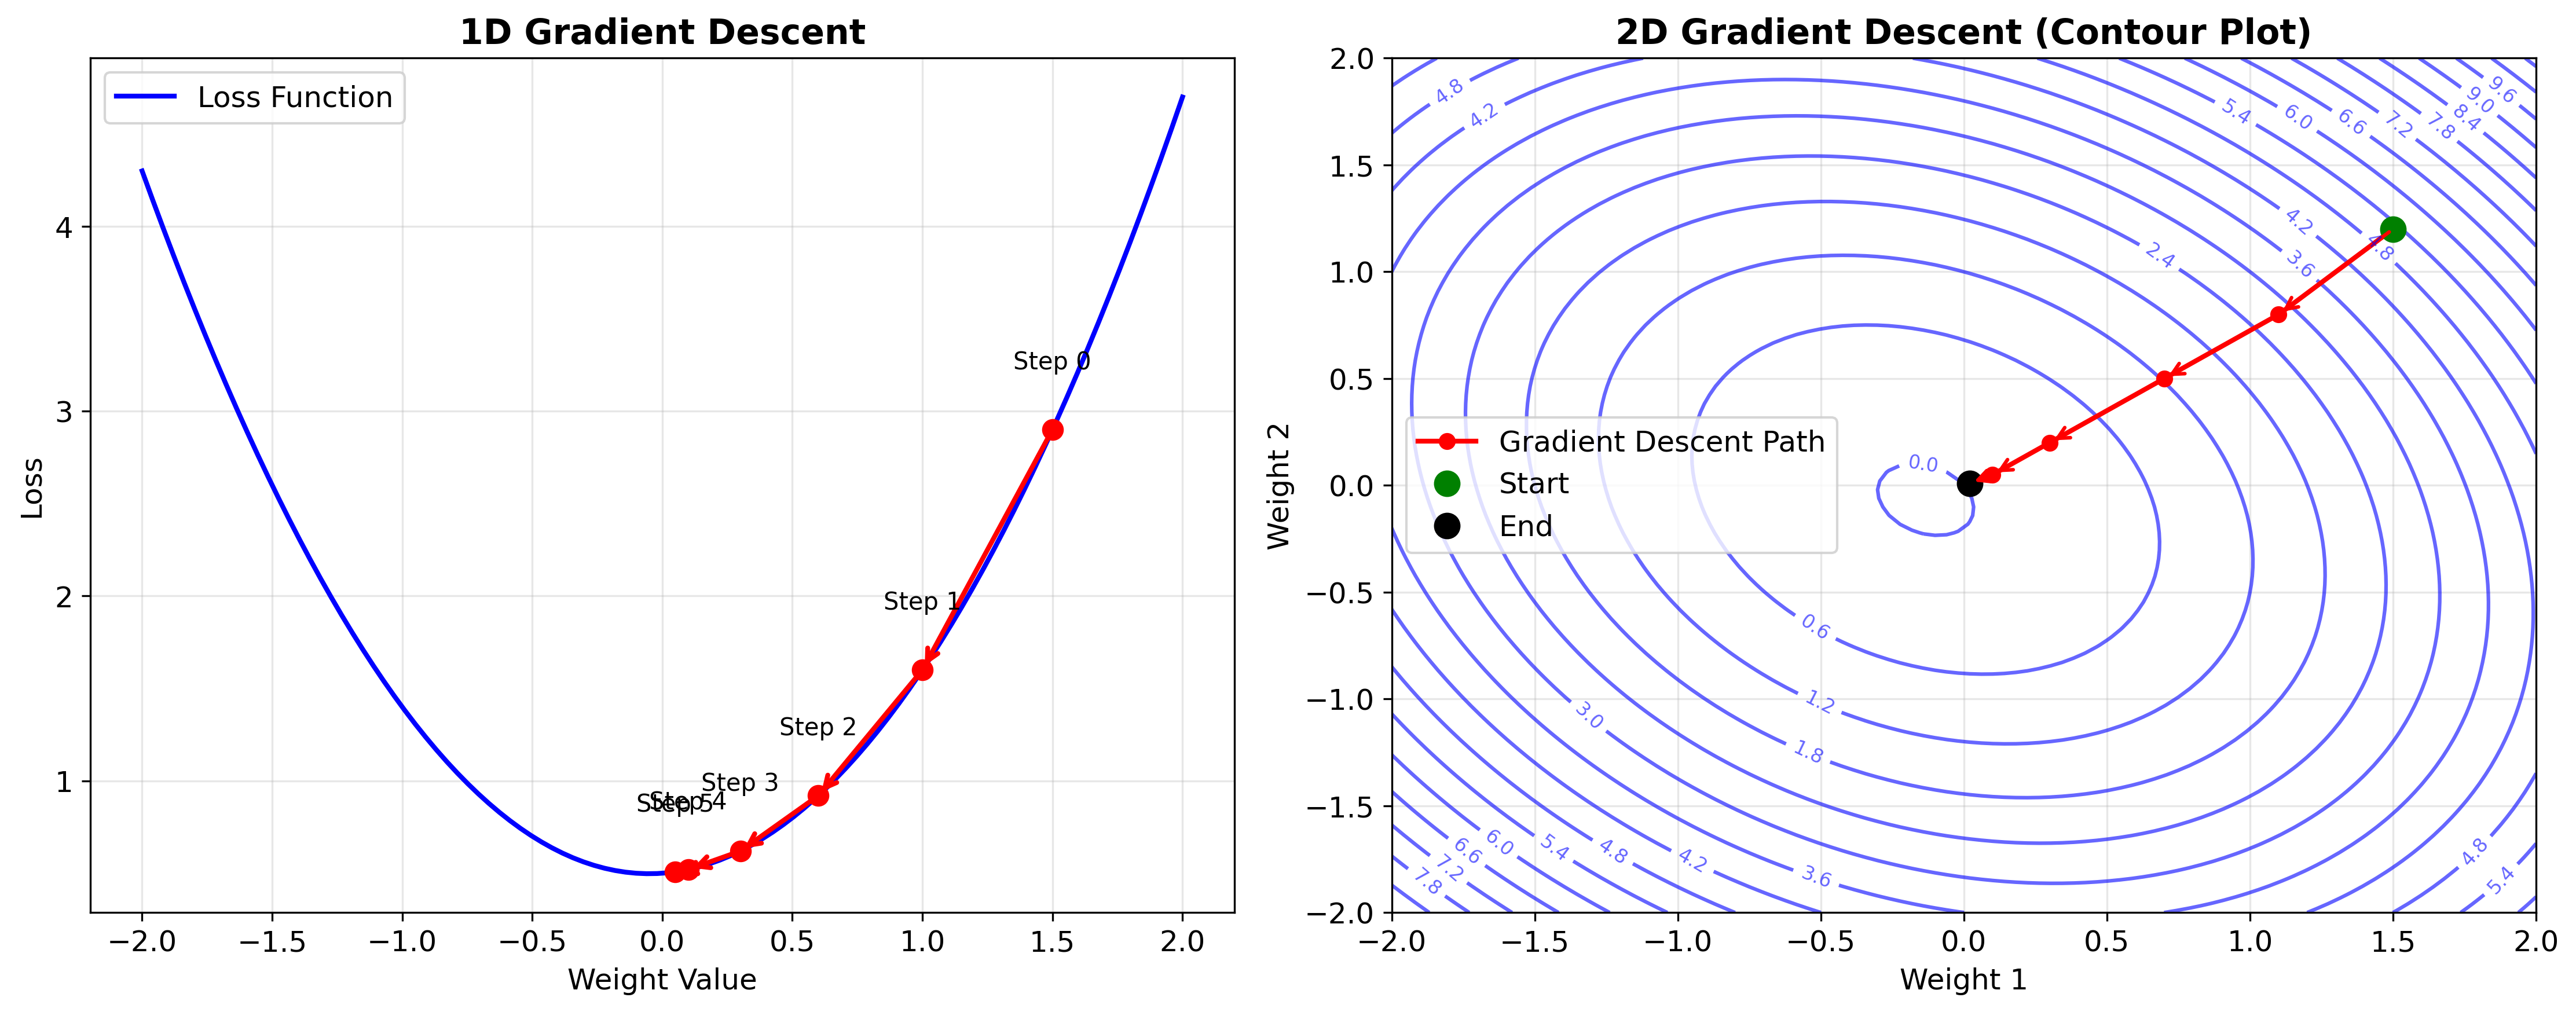
\includegraphics[width=0.8\textwidth]{../figures/gradient_descent_visualization.png}

\vspace{0.2cm}

\begin{alertblock}{Weight Update Rule}
$$\mathbf{W}^{(l)} := \mathbf{W}^{(l)} - \alpha \frac{\partial L}{\partial \mathbf{W}^{(l)}}$$
$$\mathbf{b}^{(l)} := \mathbf{b}^{(l)} - \alpha \frac{\partial L}{\partial \mathbf{b}^{(l)}}$$
where $\alpha$ is the learning rate.
\end{alertblock}
\end{frame}

% ========================================
% Section: Regularization
% ========================================

\section{Regularization Techniques}

\begin{frame}{The Overfitting Problem}
\centering
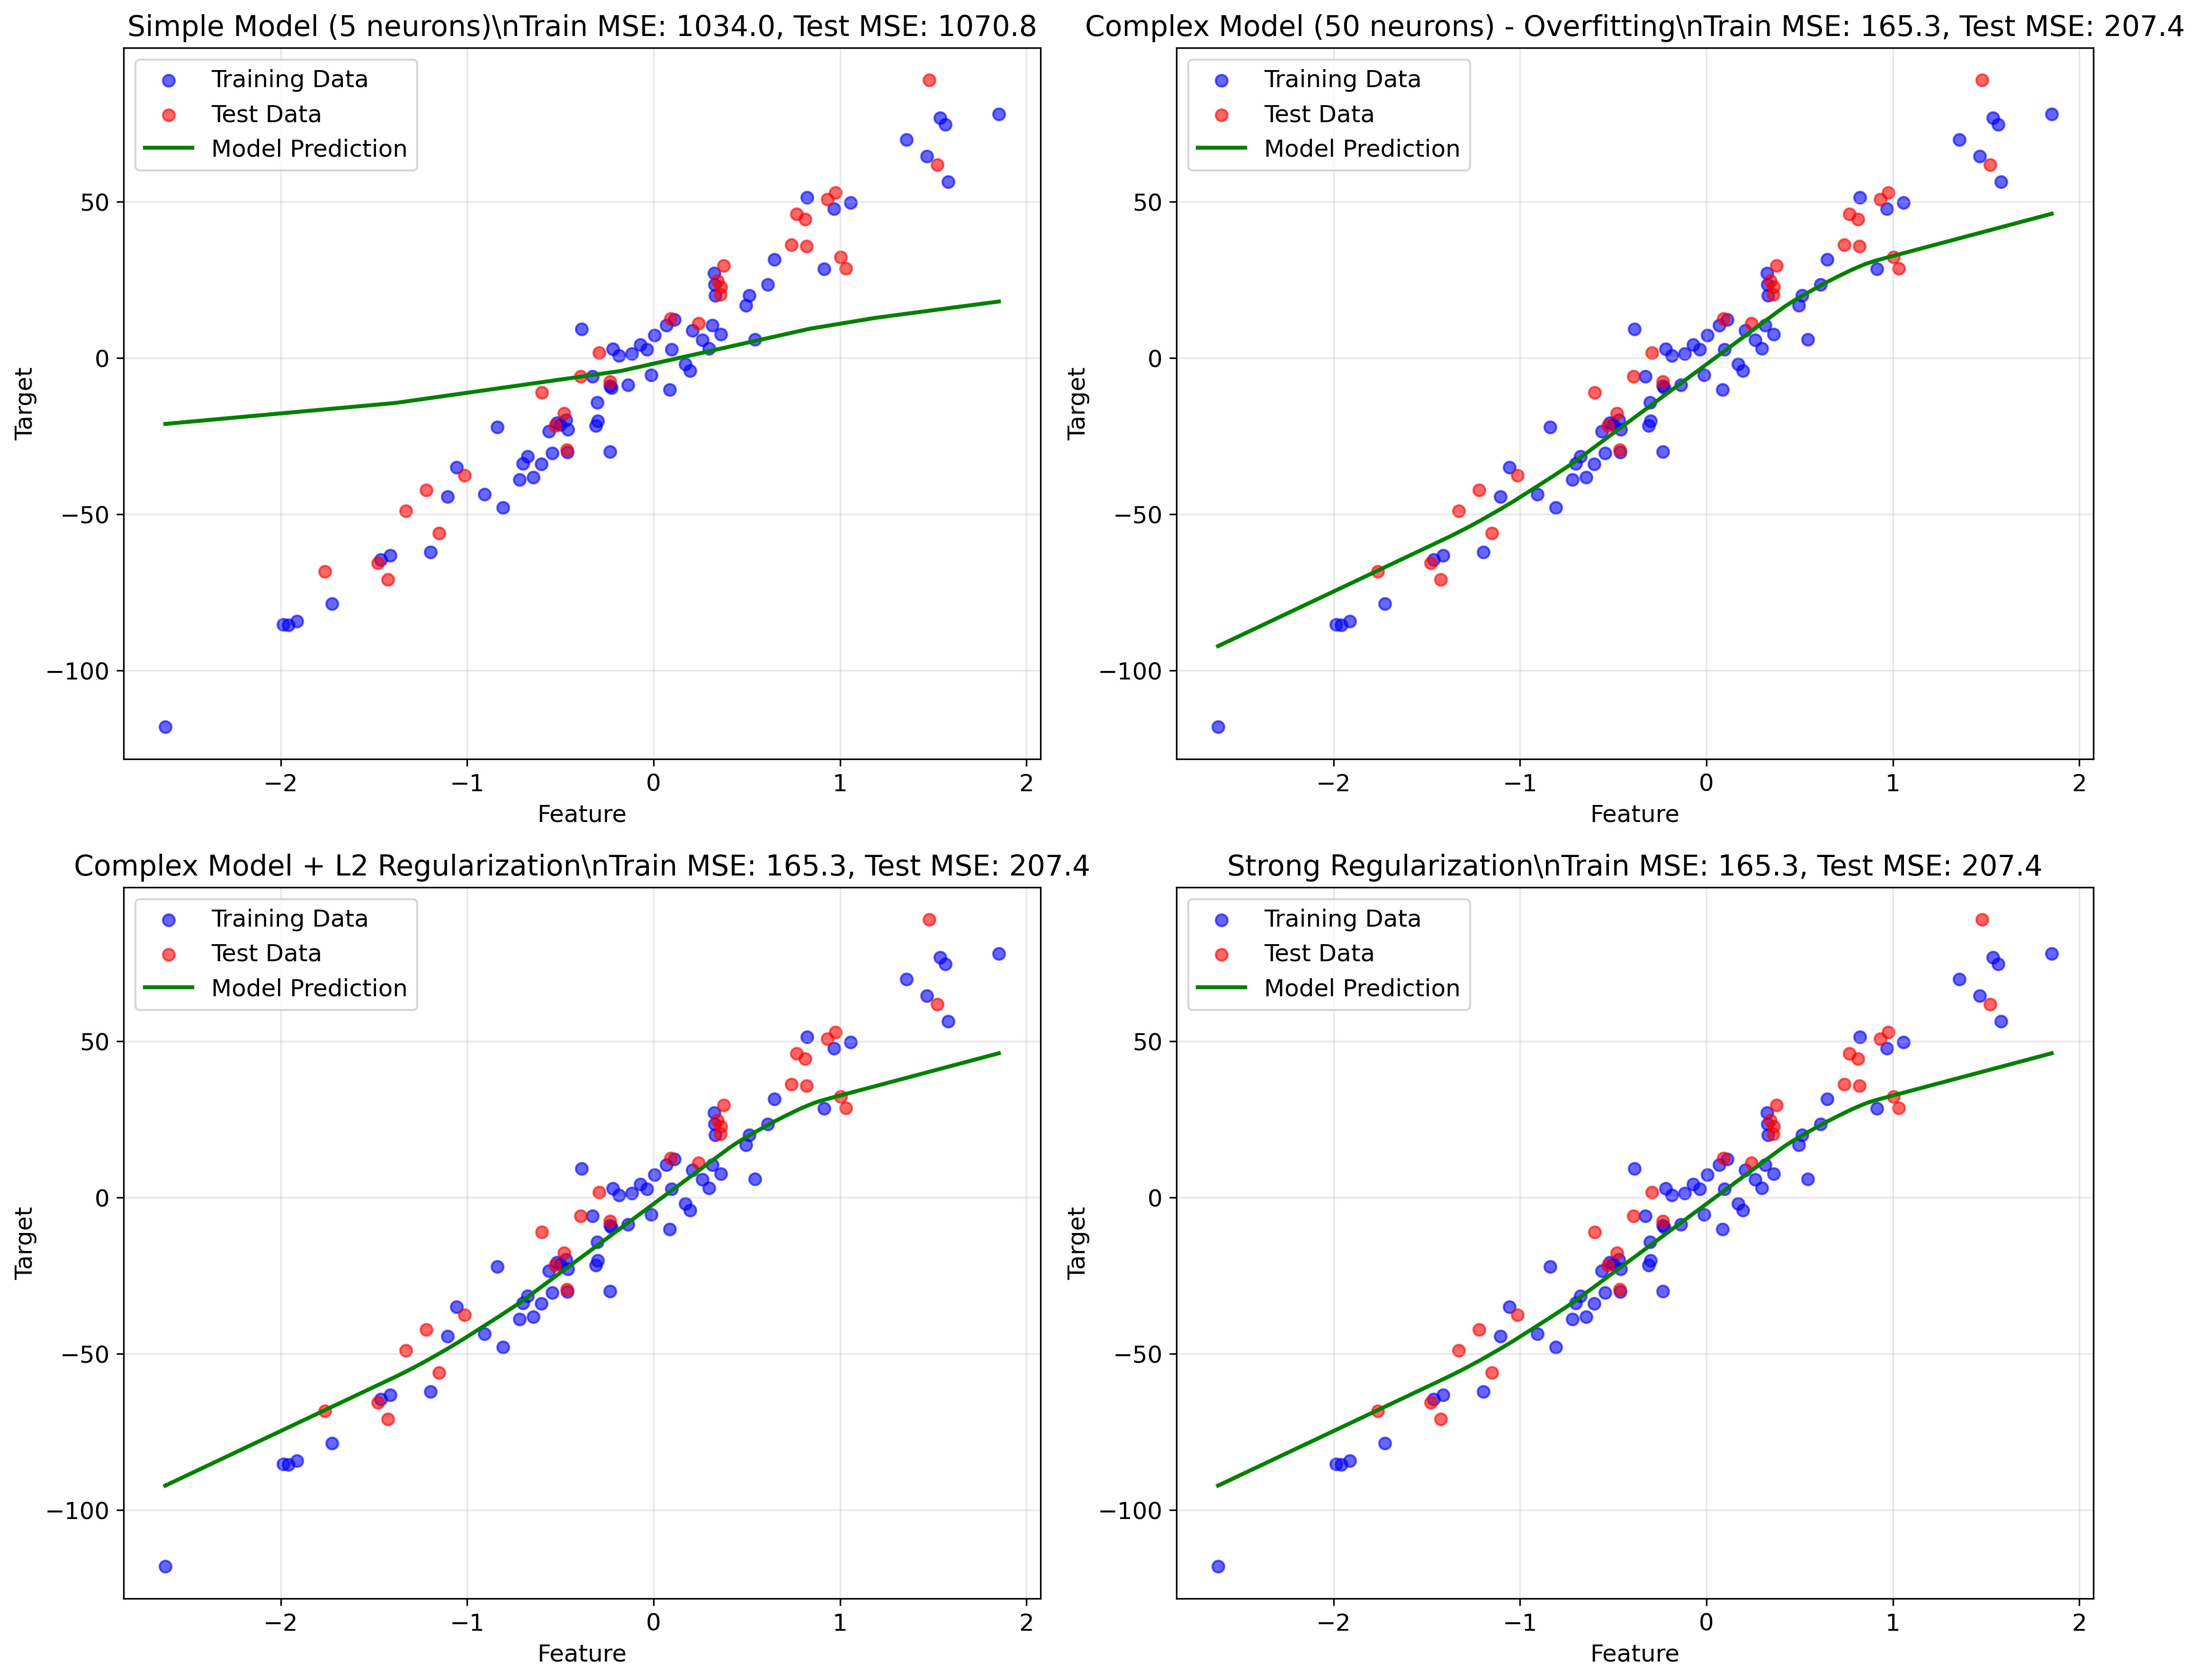
\includegraphics[width=0.7\textwidth]{../figures/overfitting_regularization_demo.png}

\vspace{0.05cm}

\begin{alertblock}{Overfitting}
Model learns training data too well, \textbf{memorizing noise} instead of generalizable patterns.
\end{alertblock}
\end{frame}

\begin{frame}{L1 and L2 Regularization}
\textbf{Add penalty terms to the loss function to control model complexity}

\vspace{0.05cm}

\begin{columns}[t]
\begin{column}{0.48\textwidth}
\begin{block}{L2 Regularization (Ridge)}
$$L_{total} = L_{data} + \lambda \sum_{l} ||\mathbf{W}^{(l)}||_2^2$$

where $||\mathbf{W}^{(l)}||_2^2 = \sum_i \sum_j (W_{ij}^{(l)})^2$

\textbf{Effect:}
\begin{itemize}
\item Shrinks weights towards zero
\item Uniform penalty on all weights
\item Smooth weight distributions
\item Preferred for most applications
\end{itemize}

\textbf{Gradient Modification:}
$$\frac{\partial L_{total}}{\partial \mathbf{W}^{(l)}} = \frac{\partial L_{data}}{\partial \mathbf{W}^{(l)}} + 2\lambda \mathbf{W}^{(l)}$$
\end{block}
\end{column}

\begin{column}{0.48\textwidth}
\begin{block}{L1 Regularization (Lasso)}
$$L_{total} = L_{data} + \lambda \sum_{l} ||\mathbf{W}^{(l)}||_1$$

where $||\mathbf{W}^{(l)}||_1 = \sum_i \sum_j |W_{ij}^{(l)}|$

\textbf{Effect:}
\begin{itemize}
\item Promotes sparsity (many weights → 0)
\item Automatic feature selection
\item Creates sparse networks
\item Useful for interpretability
\end{itemize}

\textbf{Gradient Modification:}
$$\frac{\partial L_{total}}{\partial \mathbf{W}^{(l)}} = \frac{\partial L_{data}}{\partial \mathbf{W}^{(l)}} + \lambda \text{sign}(\mathbf{W}^{(l)})$$
\end{block}
\end{column}
\end{columns}

\vspace{0.1cm}

\begin{alertblock}{Hyperparameter $\lambda$}
Controls regularization strength: \textbf{larger $\lambda$} → more regularization → simpler model
\end{alertblock}
\end{frame}

\begin{frame}{L1 vs L2 Regularization Comparison}
\centering
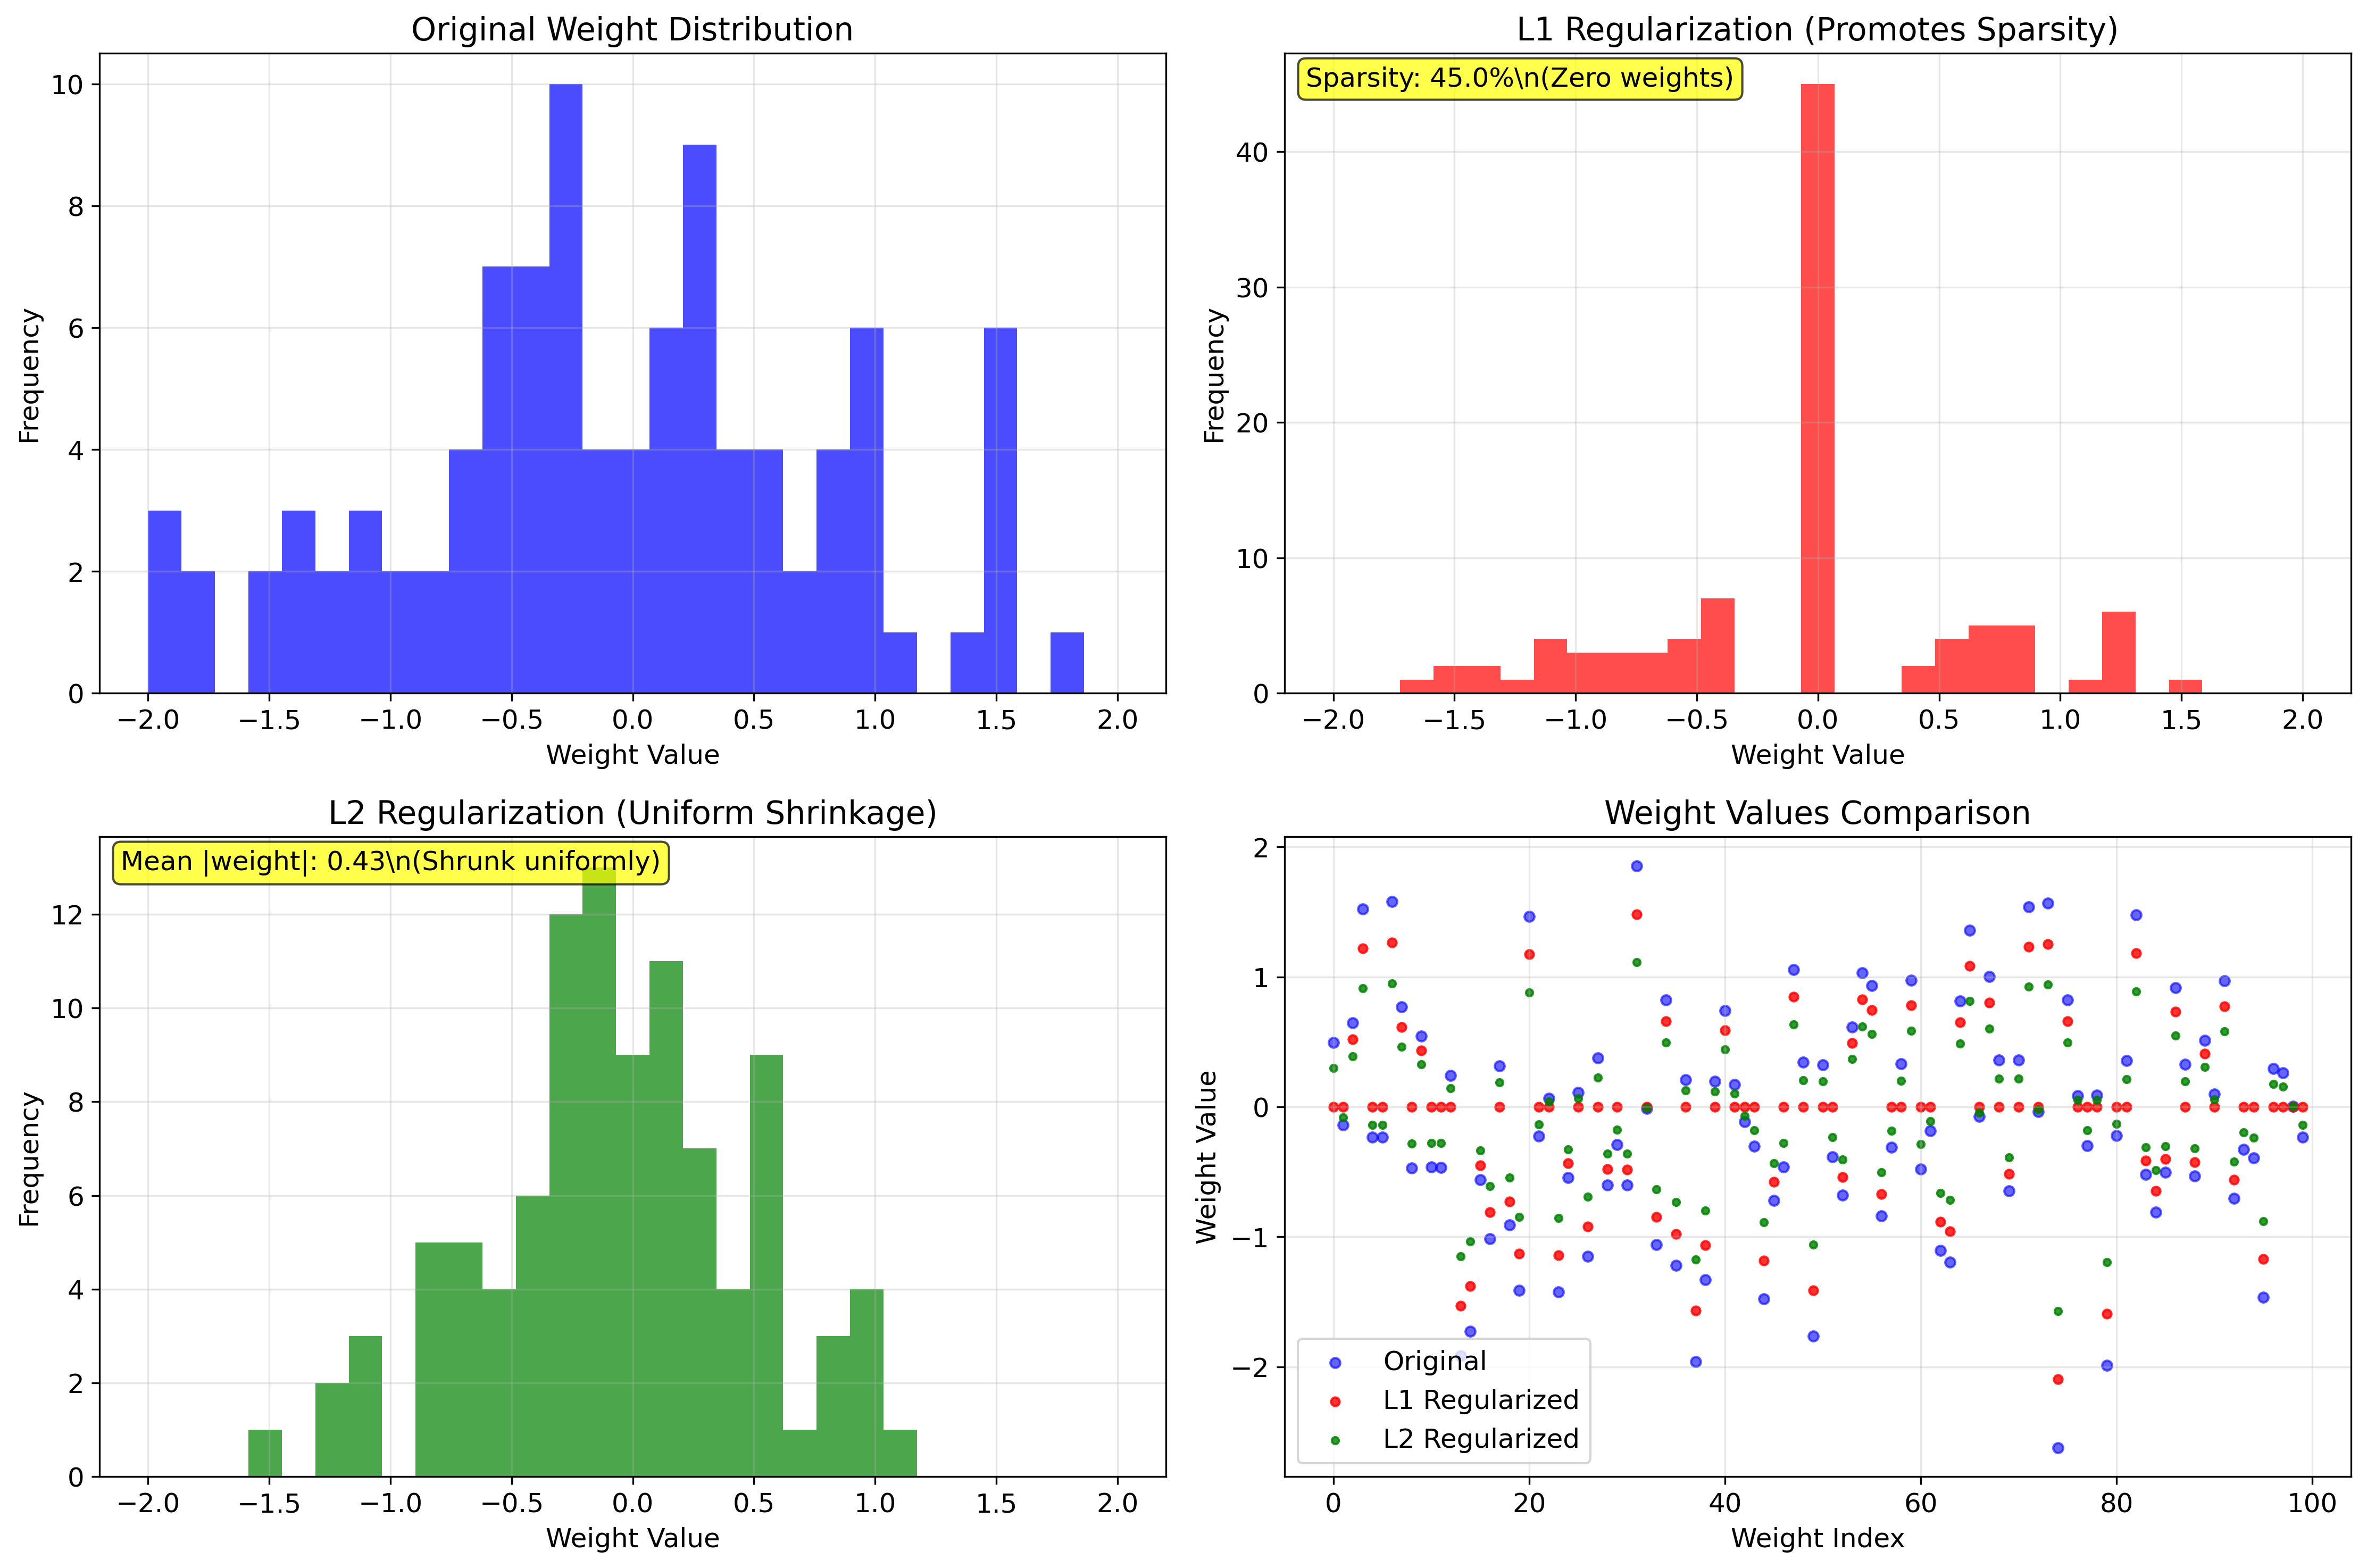
\includegraphics[width=0.65\textwidth]{../figures/l1_vs_l2_regularization.png}

\vspace{0.05cm}

\begin{columns}[t]
\begin{column}{0.48\textwidth}
\begin{block}{When to Use L2}
\begin{itemize}
\setlength{\itemsep}{1pt}
\item General-purpose regularization
\item All features potentially relevant
\item Want smooth weight shrinkage
\item Most common choice
\end{itemize}
\end{block}
\end{column}

\begin{column}{0.48\textwidth}
\begin{block}{When to Use L1}
\begin{itemize}
\setlength{\itemsep}{1pt}
\item Feature selection needed
\item Many irrelevant features
\item Want sparse models
\item Interpretability important
\end{itemize}
\end{block}
\end{column}
\end{columns}
\end{frame}

\begin{frame}{Dropout: A Different Approach}
\centering

\begin{tikzpicture}[scale=0.8, every node/.style={scale=0.8}]
    % Training network (with dropout)
    \node[above, font=\bfseries] at (2.25,3.8) {Training (with Dropout)};

    % Input layer - centered vertically
    \foreach \y in {0,1,2,3} {
        \node[input neuron] (TI-\y) at (0,{3-\y}) {$x_{\y}$};
    }

    % Hidden layer with some dropped out neurons - centered
    \node[hidden neuron] (TH-0) at (2.5,{3-0}) {};
    \node[hidden neuron, fill=gray!50, draw=gray] (TH-1) at (2.5,{3-1}) {\scriptsize X}; % Dropped out
    \node[hidden neuron] (TH-2) at (2.5,{3-2}) {};
    \node[hidden neuron, fill=gray!50, draw=gray] (TH-3) at (2.5,{3-3}) {\scriptsize X}; % Dropped out

    % Output layer - centered
    \node[output neuron] (TO) at (5,1.5) {$y$};

    % Active connections only - reduced opacity
    \draw[strong connection, opacity=0.3] (TI-0) -- (TH-0);
    \draw[strong connection, opacity=0.3] (TI-0) -- (TH-2);
    \draw[strong connection, opacity=0.3] (TI-1) -- (TH-0);
    \draw[strong connection, opacity=0.3] (TI-1) -- (TH-2);
    \draw[strong connection, opacity=0.3] (TI-2) -- (TH-0);
    \draw[strong connection, opacity=0.3] (TI-2) -- (TH-2);
    \draw[strong connection, opacity=0.3] (TI-3) -- (TH-0);
    \draw[strong connection, opacity=0.3] (TI-3) -- (TH-2);

    \draw[strong connection, opacity=0.3] (TH-0) -- (TO);
    \draw[strong connection, opacity=0.3] (TH-2) -- (TO);

    % Testing network (no dropout)
    \node[above, font=\bfseries] at (8.75,3.8) {Testing (no Dropout)};

    % Input layer - centered vertically
    \foreach \y in {0,1,2,3} {
        \node[input neuron] (EI-\y) at (6.5,{3-\y}) {$x_{\y}$};
    }

    % Hidden layer - all active, centered
    \foreach \y in {0,1,2,3} {
        \node[hidden neuron] (EH-\y) at (9,{3-\y}) {};
    }

    % Output layer - centered
    \node[output neuron] (EO) at (11.5,1.5) {$y$};

    % All connections active - very light
    \foreach \i in {0,1,2,3} {
        \foreach \j in {0,1,2,3} {
            \draw[connection, opacity=0.2] (EI-\i) -- (EH-\j);
        }
    }

    \foreach \j in {0,1,2,3} {
        \draw[connection, opacity=0.2] (EH-\j) -- (EO);
    }

    % Dropout probability label - better positioning
    \node[below, font=\footnotesize] at (2.5,-0.5) {Dropout rate: $p = 0.5$};
    \node[below, font=\footnotesize] at (9,-0.5) {All neurons active};

    % Layer labels
    \node[layer label] at (0,-1.1) {Input};
    \node[layer label] at (2.5,-1.1) {Hidden};
    \node[layer label] at (5,-1.1) {Output};

    \node[layer label] at (6.5,-1.1) {Input};
    \node[layer label] at (9,-1.1) {Hidden};
    \node[layer label] at (11.5,-1.1) {Output};
\end{tikzpicture}

\vspace{0.3cm}

\begin{alertblock}{Dropout Technique}
Randomly \textbf{set neurons to zero} during training to prevent co-adaptation and improve generalization.
\end{alertblock}
\end{frame}

\begin{frame}{Dropout: Mathematical Formulation}
\textbf{Training Phase:}
\begin{align}
\mathbf{r}^{(l)} &\sim \text{Bernoulli}(p) \quad \text{(dropout mask)} \\
\tilde{\mathbf{a}}^{(l)} &= \mathbf{r}^{(l)} \odot \mathbf{a}^{(l)} \quad \text{(apply mask)} \\
\mathbf{z}^{(l+1)} &= \mathbf{W}^{(l+1)} \tilde{\mathbf{a}}^{(l)} + \mathbf{b}^{(l+1)}
\end{align}

\textbf{Testing Phase:}
\begin{align}
\mathbf{z}^{(l+1)} &= p \cdot \mathbf{W}^{(l+1)} \mathbf{a}^{(l)} + \mathbf{b}^{(l+1)} \quad \text{(scale weights)}
\end{align}

\vspace{0.1cm}

\begin{columns}[t]
\begin{column}{0.48\textwidth}
\begin{block}{Dropout Benefits}
\begin{itemize}
\setlength{\itemsep}{0pt}
\item \textbf{Prevents overfitting:} Reduces complex co-adaptations
\item \textbf{Model averaging:} Approximates ensemble of networks
\item \textbf{Robust features:} Forces redundant representations
\item \textbf{Easy to implement:} Simple modification to forward pass
\end{itemize}
\vspace{0.05cm}
\textbf{Typical rates:} 0.2-0.5 for hidden layers, 0.1-0.2 for input
\end{block}
\end{column}

\begin{column}{0.48\textwidth}
\begin{exampleblock}{Implementation Notes}
\textbf{Training vs Testing:}
\begin{itemize}
\setlength{\itemsep}{0pt}
\item Training: Randomly drop neurons
\item Testing: Use all neurons but scale outputs
\item Modern frameworks handle this automatically
\end{itemize}
\vspace{0.05cm}
\textbf{Why Scaling Works:}
\begin{itemize}
\setlength{\itemsep}{0pt}
\item Training: Each neuron is "on" with probability $p$
\item Testing: All neurons are "on"
\item Scaling by $p$ maintains expected activation levels
\end{itemize}
\end{exampleblock}
\end{column}
\end{columns}
\begin{alertblock}{Best Practice}
Use dropout in \textbf{hidden layers only}, not in output layer. Start with rate 0.5 and tune.
\end{alertblock}
\end{frame}

\begin{frame}{Regularization Comparison}
\centering
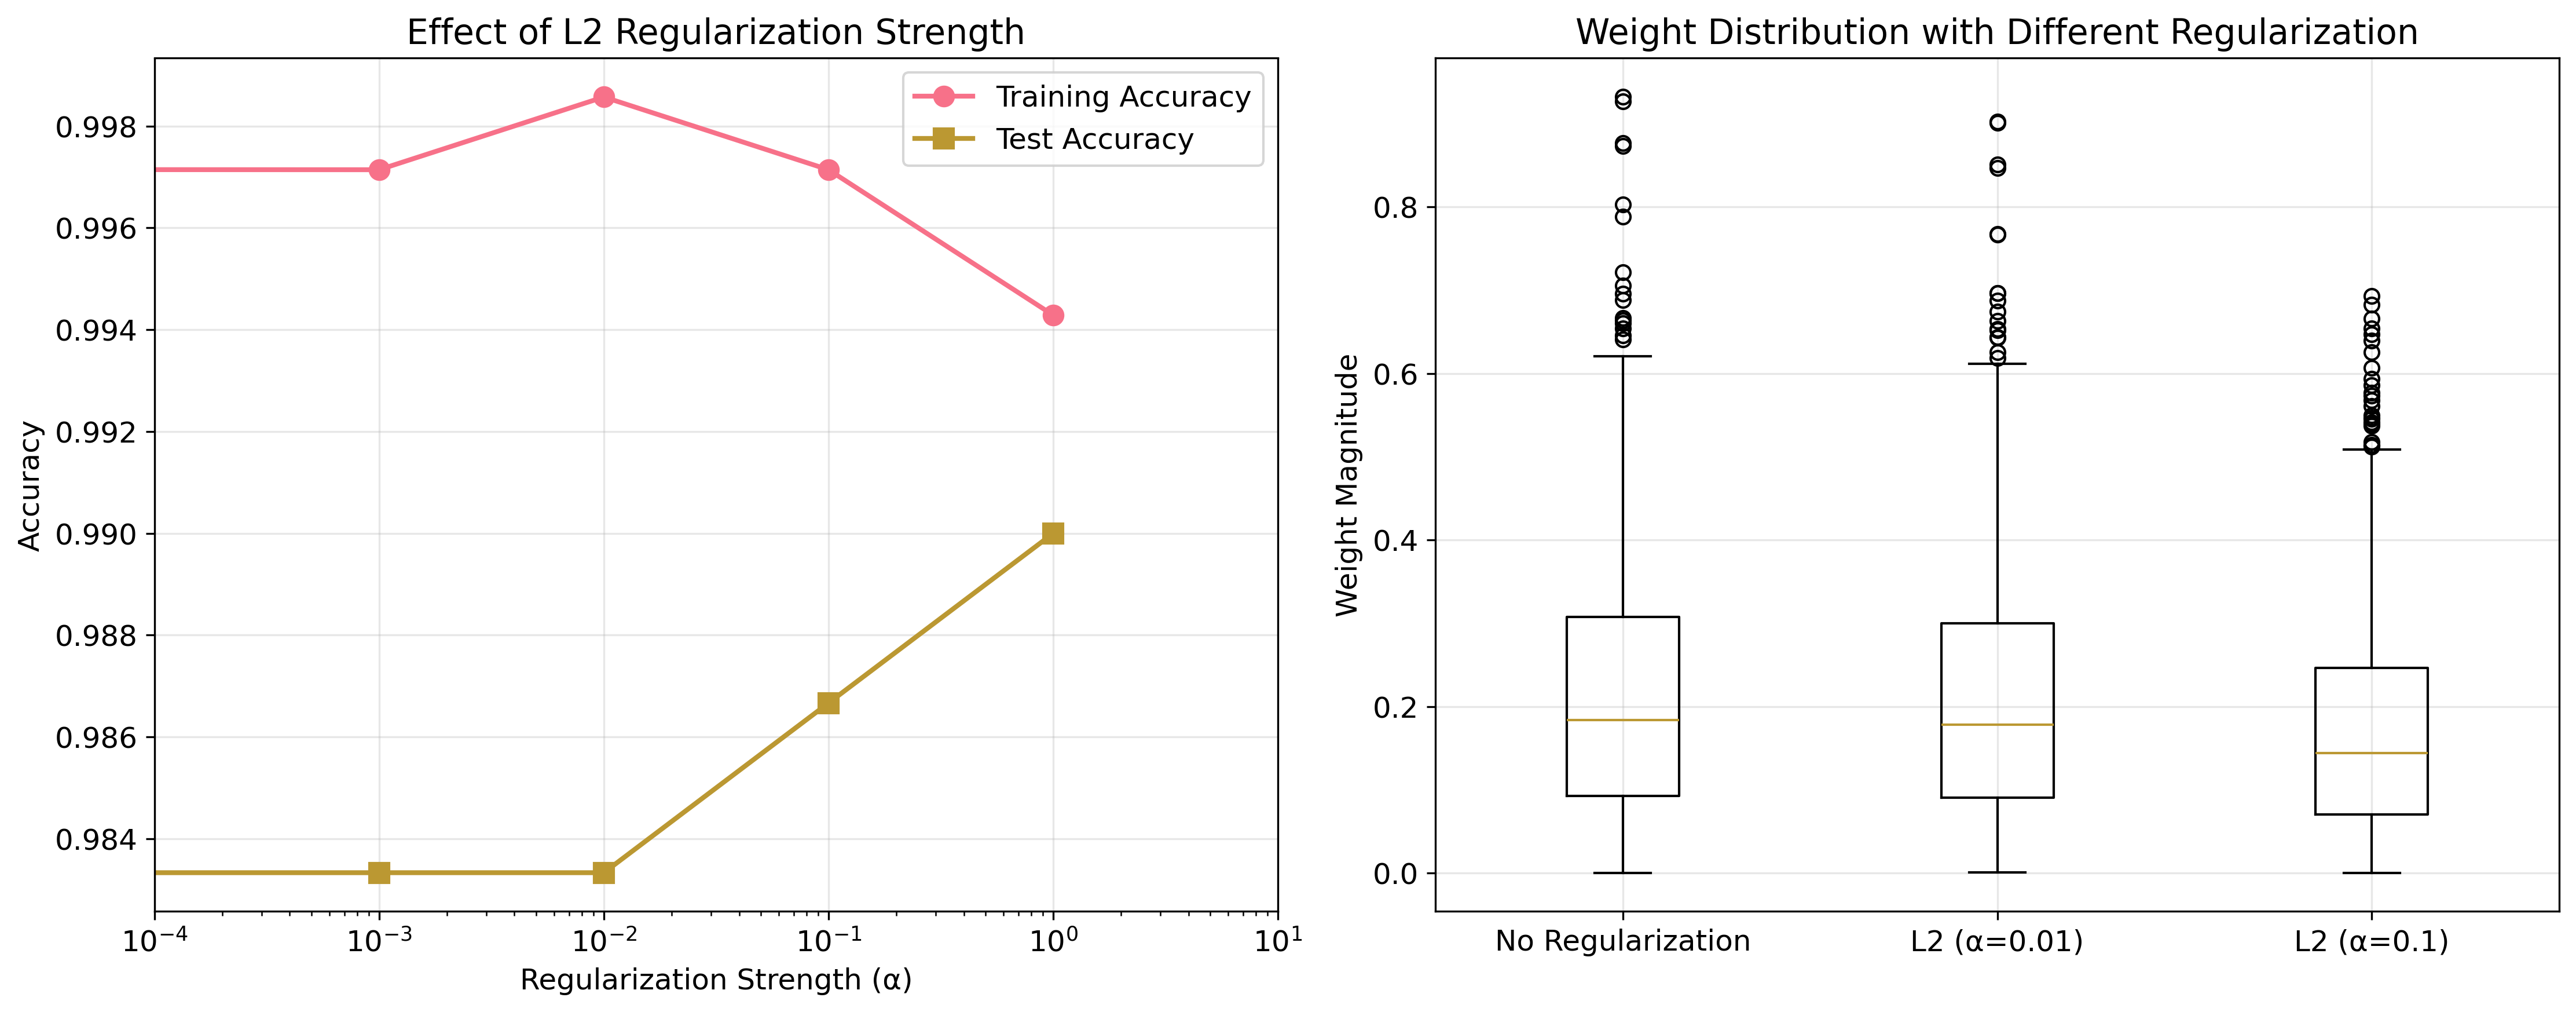
\includegraphics[width=0.75\textwidth]{../figures/regularization_comparison.png}

\vspace{0.05cm}

\begin{columns}[t]
\begin{column}{0.48\textwidth}
\begin{block}{Choosing Regularization}
\textbf{Start with:}
\begin{itemize}
\setlength{\itemsep}{1pt}
\item L2 regularization ($\lambda = 0.01$)
\item Dropout (rate = 0.5)
\item Early stopping
\end{itemize}

\textbf{If still overfitting:}
\begin{itemize}
\setlength{\itemsep}{1pt}
\item Increase regularization strength
\item Add more dropout
\item Reduce model complexity
\end{itemize}
\end{block}
\end{column}

\begin{column}{0.48\textwidth}
\begin{block}{Other Techniques}
\textbf{Early Stopping:}
\begin{itemize}
\setlength{\itemsep}{1pt}
\item Monitor validation loss
\item Stop when it starts increasing
\item Simple and effective
\end{itemize}

\textbf{Data Augmentation:}
\begin{itemize}
\setlength{\itemsep}{1pt}
\item Artificially increase training data
\item Add noise, rotations, etc.
\item Domain-specific techniques
\end{itemize}
\end{block}
\end{column}
\end{columns}
\end{frame}

\begin{frame}{Training Curves with Regularization}
\centering
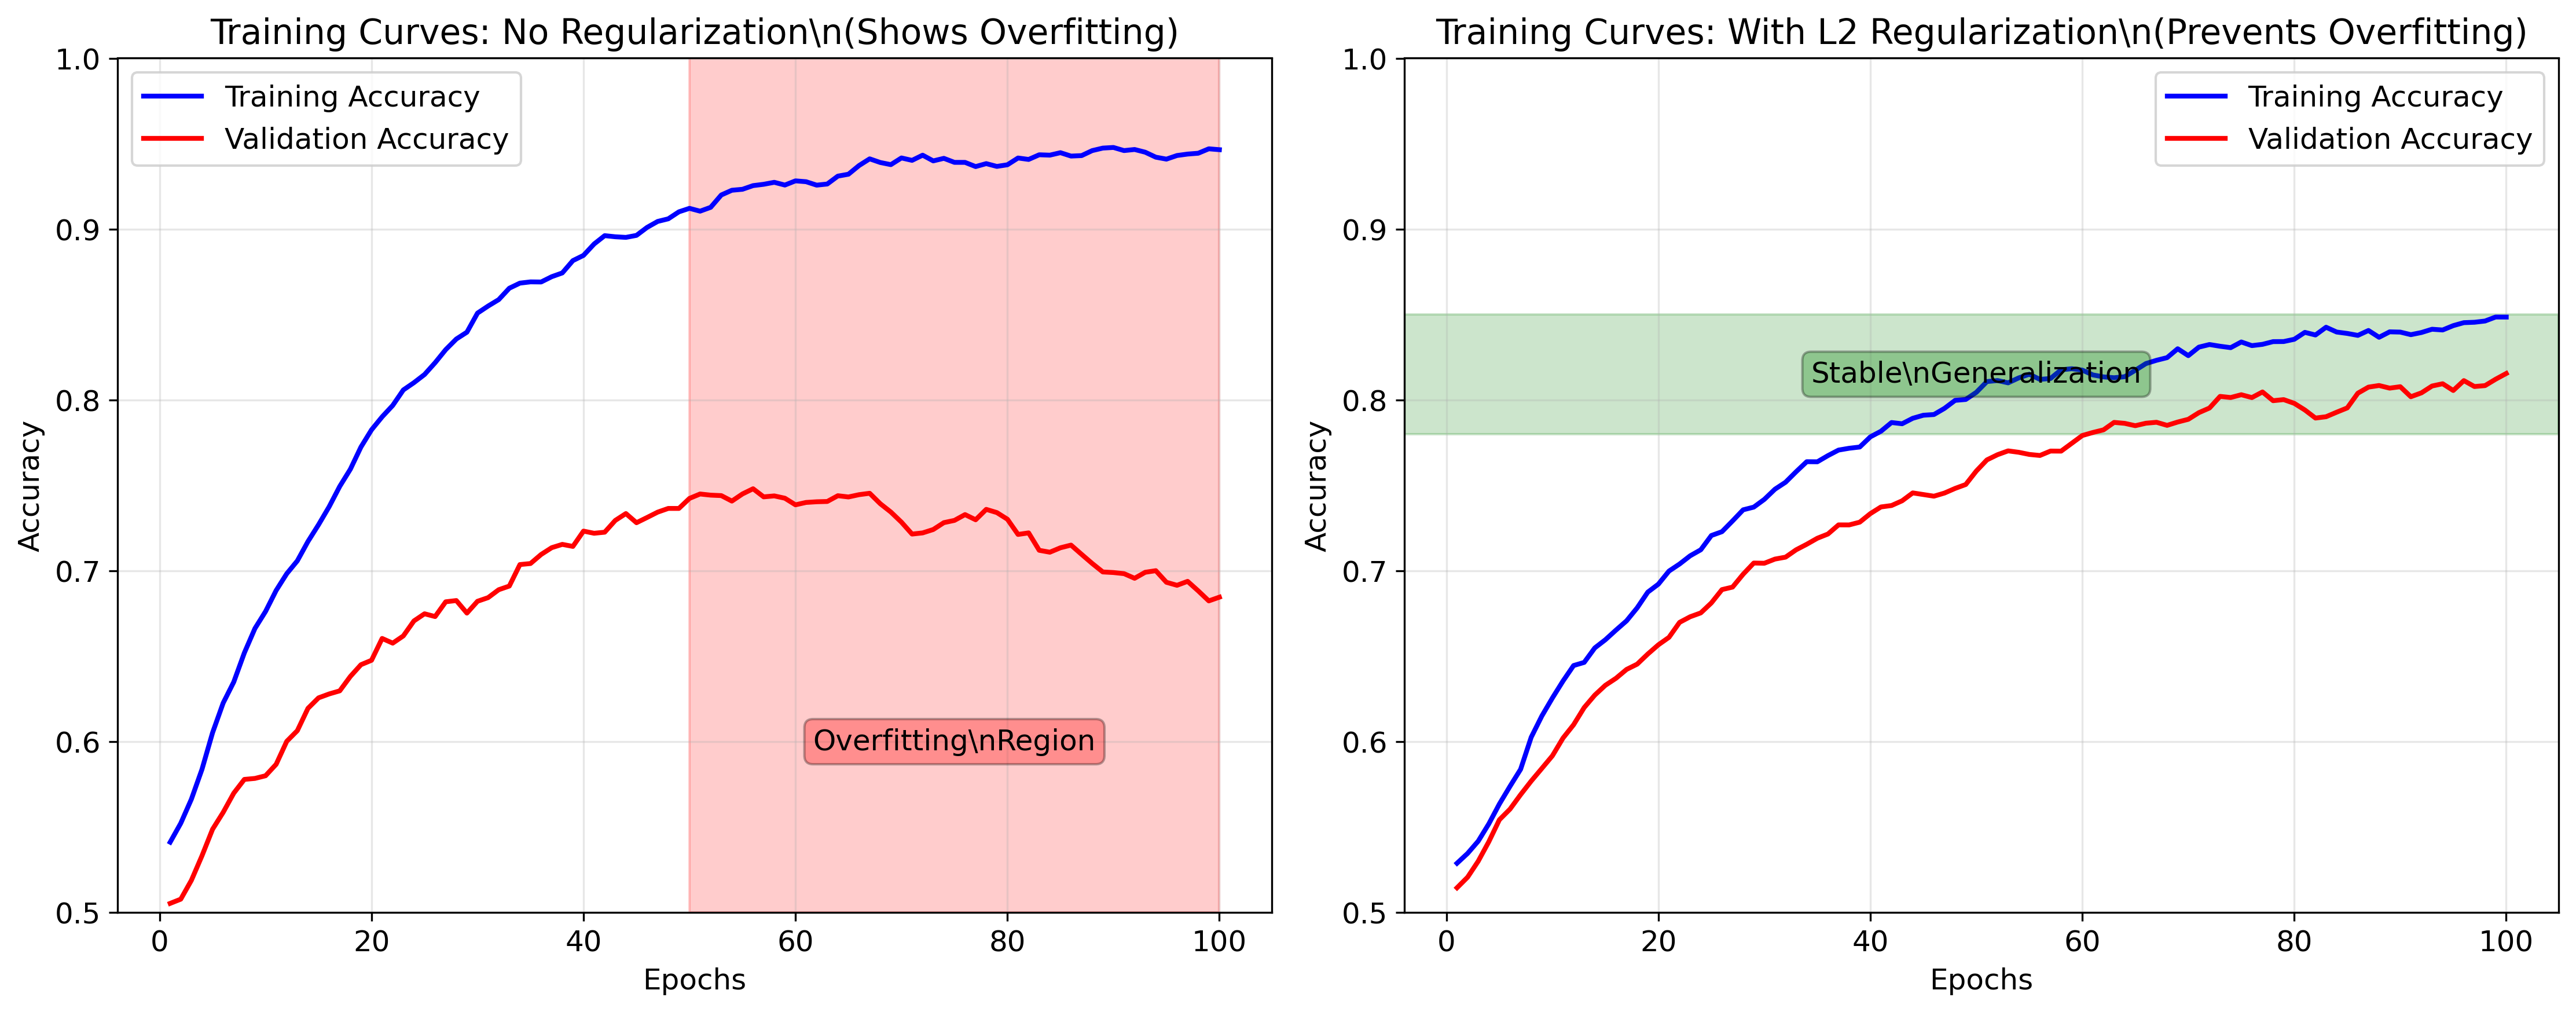
\includegraphics[width=0.75\textwidth]{../figures/training_curves_regularization.png}

\vspace{0.05cm}

\begin{alertblock}{Monitoring Training}
Use \textbf{validation curves} to detect overfitting and choose regularization strength.
\end{alertblock}
\end{frame}

% ========================================
% Section: Best Practices
% ========================================

\section{Training Best Practices}

\begin{frame}{Weight Initialization}
\textbf{Proper initialization is crucial for successful training}

\vspace{0.3cm}

\begin{columns}[t]
\begin{column}{0.48\textwidth}
\begin{block}{Poor Initialization}
\textbf{All zeros:} No learning (symmetry)
$$W_{ij} = 0 \Rightarrow \text{no gradient flow}$$

\textbf{Too large:} Exploding gradients
$$W_{ij} \sim \mathcal{N}(0, 1) \Rightarrow \text{saturation}$$

\textbf{Too small:} Vanishing gradients
$$W_{ij} \sim \mathcal{N}(0, 0.01) \Rightarrow \text{weak signals}$$
\end{block}
\end{column}

\begin{column}{0.48\textwidth}
\begin{block}{Good Initialization}
\textbf{Xavier/Glorot (Sigmoid/Tanh):}
$$W_{ij} \sim \mathcal{N}\left(0, \sqrt{\frac{2}{n_{in} + n_{out}}}\right)$$

\textbf{He initialization (ReLU):}
$$W_{ij} \sim \mathcal{N}\left(0, \sqrt{\frac{2}{n_{in}}}\right)$$

\textbf{Bias initialization:}
$$b_i = 0 \text{ (usually sufficient)}$$
\end{block}
\end{column}
\end{columns}

\vspace{0.3cm}

\begin{alertblock}{\textbf{Why These Work}}
Maintain \textbf{activation variance} and \textbf{gradient variance} across layers during initialization.
\end{alertblock}
\end{frame}

\begin{frame}{Learning Rate and Optimization}
\begin{columns}[t]
\begin{column}{0.48\textwidth}
\begin{block}{Learning Rate Selection}
\textbf{Too high:} Overshooting, instability
\begin{itemize}
\item Loss explodes or oscillates
\item Network doesn't converge
\item Weights become very large
\end{itemize}

\textbf{Too low:} Slow convergence
\begin{itemize}
\item Training takes forever
\item Gets stuck in local minima
\item Poor final performance
\end{itemize}

\textbf{Good range:} Typically $10^{-4}$ to $10^{-1}$
\end{block}
\end{column}

\begin{column}{0.48\textwidth}
\begin{block}{Advanced Optimizers}
\textbf{SGD with Momentum:}
$$\mathbf{v}_t = \beta \mathbf{v}_{t-1} + (1-\beta) \nabla L$$
$$\mathbf{W} := \mathbf{W} - \alpha \mathbf{v}_t$$

\textbf{Adam (Adaptive Moments):}
\begin{align}
\mathbf{m}_t &= \beta_1 \mathbf{m}_{t-1} + (1-\beta_1) \nabla L \\
\mathbf{v}_t &= \beta_2 \mathbf{v}_{t-1} + (1-\beta_2) (\nabla L)^2 \\
\mathbf{W} &:= \mathbf{W} - \alpha \frac{\mathbf{m}_t}{\sqrt{\mathbf{v}_t} + \epsilon}
\end{align}

\textbf{Default choice:} Adam with $\alpha = 0.001$
\end{block}
\end{column}
\end{columns}

\vspace{0.3cm}

\begin{alertblock}{Learning Rate Scheduling}
\textbf{Decay strategies:} Step decay, exponential decay, cosine annealing. Start high, reduce during training.
\end{alertblock}
\end{frame}

\begin{frame}{Training Diagnostics}
\textbf{Monitor these metrics during training:}

\vspace{0.3cm}

\begin{columns}[t]
\begin{column}{0.48\textwidth}
\begin{block}{Loss Monitoring}
\begin{itemize}
\item \textbf{Training loss}: Should decrease monotonically
\item \textbf{Validation loss}: Should decrease, then stabilize
\item \textbf{Gap}: Indicates overfitting if too large
\end{itemize}

\textbf{Warning Signs:}
\begin{itemize}
\item Loss increases: Learning rate too high
\item Loss plateaus early: Learning rate too low
\item Validation loss increases: Overfitting
\end{itemize}
\end{block}

\begin{block}{Gradient Monitoring}
\begin{itemize}
\item \textbf{Gradient norms}: Should be reasonable ($10^{-6}$ to $10^{-1}$)
\item \textbf{Vanishing}: Gradients → 0 in early layers
\item \textbf{Exploding}: Gradients become very large
\end{itemize}
\end{block}
\end{column}

\begin{column}{0.48\textwidth}
\begin{block}{Activation Monitoring}
\begin{itemize}
\item \textbf{Activation statistics}: Mean, std, sparsity
\item \textbf{Dead neurons}: Always output zero
\item \textbf{Saturated neurons}: Always in saturation region
\end{itemize}

\textbf{Healthy activations:}
\begin{itemize}
\item Reasonable variance (not too small/large)
\item Some sparsity (for ReLU)
\item No layers completely dead
\end{itemize}
\end{block}

\begin{block}{Weight Monitoring}
\begin{itemize}
\item \textbf{Weight distributions}: Should be reasonable
\item \textbf{Weight updates}: $|\Delta W| / |W| \approx 10^{-3}$
\item \textbf{Layer-wise learning rates}: May need adjustment
\end{itemize}
\end{block}
\end{column}
\end{columns}

\begin{alertblock}{Tools}
Use \textbf{TensorBoard}, \textbf{Weights \& Biases}, or similar tools for comprehensive monitoring and visualization.
\end{alertblock}
\end{frame}

\begin{frame}{Common Problems and Solutions}
\begin{columns}[t]
\begin{column}{0.48\textwidth}
\begin{block}{Problem: Vanishing Gradients}
\textbf{Symptoms:}
\begin{itemize}
\setlength{\itemsep}{0pt}
\item Early layers don't learn
\item Gradients approach zero
\end{itemize}
\textbf{Solutions:}
\begin{itemize}
\setlength{\itemsep}{0pt}
\item Use ReLU activations
\item Proper weight initialization
\item Batch normalization
\end{itemize}
\end{block}
\begin{block}{Problem: Overfitting}
\textbf{Symptoms:}
\begin{itemize}
\setlength{\itemsep}{0pt}
\item Training accuracy >> validation accuracy
\item Validation loss increases
\end{itemize}
\textbf{Solutions:}
\begin{itemize}
\setlength{\itemsep}{0pt}
\item Add regularization (L2, dropout)
\item Reduce model complexity
\item More training data
\end{itemize}
\end{block}
\end{column}

\begin{column}{0.48\textwidth}
\begin{block}{Problem: Exploding Gradients}
\textbf{Symptoms:}
\begin{itemize}
\setlength{\itemsep}{0pt}
\item Loss becomes NaN
\item Weights blow up
\end{itemize}
\textbf{Solutions:}
\begin{itemize}
\setlength{\itemsep}{0pt}
\item Gradient clipping
\item Lower learning rate
\item Better initialization
\end{itemize}
\end{block}
\begin{block}{Problem: Slow Convergence}
\textbf{Symptoms:}
\begin{itemize}
\setlength{\itemsep}{0pt}
\item Loss decreases slowly
\item Gets stuck in plateaus
\end{itemize}
\textbf{Solutions:}
\begin{itemize}
\setlength{\itemsep}{0pt}
\item Increase learning rate
\item Use adaptive optimizers
\end{itemize}
\end{block}
\end{column}
\end{columns}
\end{frame}

% ========================================
% Section: Summary
% ========================================

\section{Summary \& Applications}

\begin{frame}{Neural Networks: Key Takeaways}
\begin{columns}[t]
\begin{column}{0.48\textwidth}
\begin{block}{Core Concepts}
\begin{itemize}
\setlength{\itemsep}{3pt}
\item \textbf{Perceptron}: Basic building block
\item \textbf{Multi-layer}: Enable complex mappings
\item \textbf{Activation functions}: Provide non-linearity
\item \textbf{Forward propagation}: Compute predictions
\item \textbf{Backpropagation}: Compute gradients efficiently
\item \textbf{Regularization}: Prevent overfitting
\end{itemize}
\end{block}

\begin{block}{Mathematical Foundation}
\begin{itemize}
\setlength{\itemsep}{2pt}
\item Matrix operations for efficiency
\item Chain rule for gradient computation
\item Optimization theory for training
\item Probability theory for interpretation
\end{itemize}
\end{block}
\end{column}

\begin{column}{0.48\textwidth}
\begin{block}{Best Practices}
\begin{itemize}
\setlength{\itemsep}{3pt}
\item \textbf{Architecture}: Start simple, add complexity gradually
\item \textbf{Initialization}: Xavier/He for proper gradient flow
\item \textbf{Optimization}: Adam optimizer with proper learning rate
\item \textbf{Regularization}: L2 + Dropout for generalization
\item \textbf{Monitoring}: Track loss, gradients, activations
\item \textbf{Debugging}: Systematic approach to problems
\end{itemize}
\end{block}

\begin{block}{When to Use Neural Networks}
\begin{itemize}
\setlength{\itemsep}{2pt}
\item Large datasets available
\item Complex non-linear patterns
\item End-to-end learning desired
\item Feature engineering is difficult
\end{itemize}
\end{block}
\end{column}
\end{columns}

\begin{alertblock}{Modern Deep Learning}
These fundamentals scale to modern architectures: \textbf{CNNs, RNNs, Transformers, ResNets, etc.}
\end{alertblock}
\end{frame}

\begin{frame}{Applications \& Real-World Impact}
\begin{columns}[t]
\begin{column}{0.48\textwidth}
\begin{block}{Computer Vision}
\begin{itemize}
\item \textbf{Image classification}: ResNet, EfficientNet
\item \textbf{Object detection}: YOLO, R-CNN
\item \textbf{Segmentation}: U-Net, Mask R-CNN
\item \textbf{Face recognition}: DeepFace, FaceNet
\item \textbf{Medical imaging}: Cancer detection, radiology
\end{itemize}
\end{block}

\begin{block}{Natural Language Processing}
\begin{itemize}
\item \textbf{Language models}: GPT, BERT, T5
\item \textbf{Translation}: Google Translate, DeepL
\item \textbf{Chatbots}: ChatGPT, virtual assistants
\item \textbf{Text analysis}: Sentiment, summarization
\end{itemize}
\end{block}
\end{column}

\begin{column}{0.48\textwidth}
\begin{block}{Other Domains}
\begin{itemize}
\item \textbf{Speech}: Recognition, synthesis, processing
\item \textbf{Recommendation}: Netflix, Amazon, Spotify
\item \textbf{Games}: AlphaGo, OpenAI Five, StarCraft
\item \textbf{Robotics}: Control, perception, planning
\item \textbf{Finance}: Trading, fraud detection, risk
\item \textbf{Science}: Drug discovery, climate modeling
\end{itemize}
\end{block}

\begin{block}{Emerging Areas}
\begin{itemize}
\item \textbf{Generative AI}: DALL-E, Midjourney, Stable Diffusion
\item \textbf{Multimodal}: CLIP, GPT-4V
\item \textbf{Reinforcement Learning}: Autonomous systems
\item \textbf{Scientific Computing}: Physics, chemistry, biology
\end{itemize}
\end{block}
\end{column}
\end{columns}

\begin{alertblock}{Impact}
Neural networks have \textbf{revolutionized AI} and are now fundamental to most modern machine learning applications.
\end{alertblock}
\end{frame}

\begin{frame}{Looking Forward: Advanced Topics}
\textbf{What's Next After This Foundation?}

\vspace{0.3cm}

\begin{columns}[t]
\begin{column}{0.48\textwidth}
\begin{block}{Specialized Architectures}
\begin{itemize}
\item \textbf{Convolutional Neural Networks (CNNs)}
  \begin{itemize}
  \item Spatial structure exploitation
  \item Translation invariance
  \item Computer vision applications
  \end{itemize}
\item \textbf{Recurrent Neural Networks (RNNs)}
  \begin{itemize}
  \item Sequential data processing
  \item Memory and temporal dynamics
  \item LSTM, GRU variants
  \end{itemize}
\item \textbf{Transformer Networks}
  \begin{itemize}
  \item Attention mechanisms
  \item Parallel processing
  \item Modern NLP backbone
  \end{itemize}
\end{itemize}
\end{block}
\end{column}

\begin{column}{0.48\textwidth}
\begin{block}{Advanced Techniques}
\begin{itemize}
\item \textbf{Batch Normalization}
  \begin{itemize}
  \item Internal covariate shift
  \item Training acceleration
  \end{itemize}
\item \textbf{Residual Connections}
  \begin{itemize}
  \item Very deep networks
  \item Gradient flow improvement
  \end{itemize}
\item \textbf{Attention Mechanisms}
  \begin{itemize}
  \item Selective focus
  \item Long-range dependencies
  \end{itemize}
\item \textbf{Generative Models}
  \begin{itemize}
  \item VAEs, GANs, Diffusion
  \item Creative AI applications
  \end{itemize}
\end{itemize}
\end{block}
\end{column}
\end{columns}

\vspace{0.3cm}

\begin{alertblock}{Next Steps}
\textbf{Practice implementation}, experiment with \textbf{real datasets}, and explore \textbf{specialized architectures} for your domain of interest.
\end{alertblock}
\end{frame}

\begin{frame}[standout]
Questions?
\end{frame}

\end{document}